\documentclass[a4paper]{article}

\usepackage{graphicx}
\usepackage{subcaption}
\usepackage[margin=.5in]{geometry}

\begin{document}

\section*{Miniature Lamp - Build Documentation}
Here are some pictures to help guide the build process:

\begin{figure}[h!]
\centerline{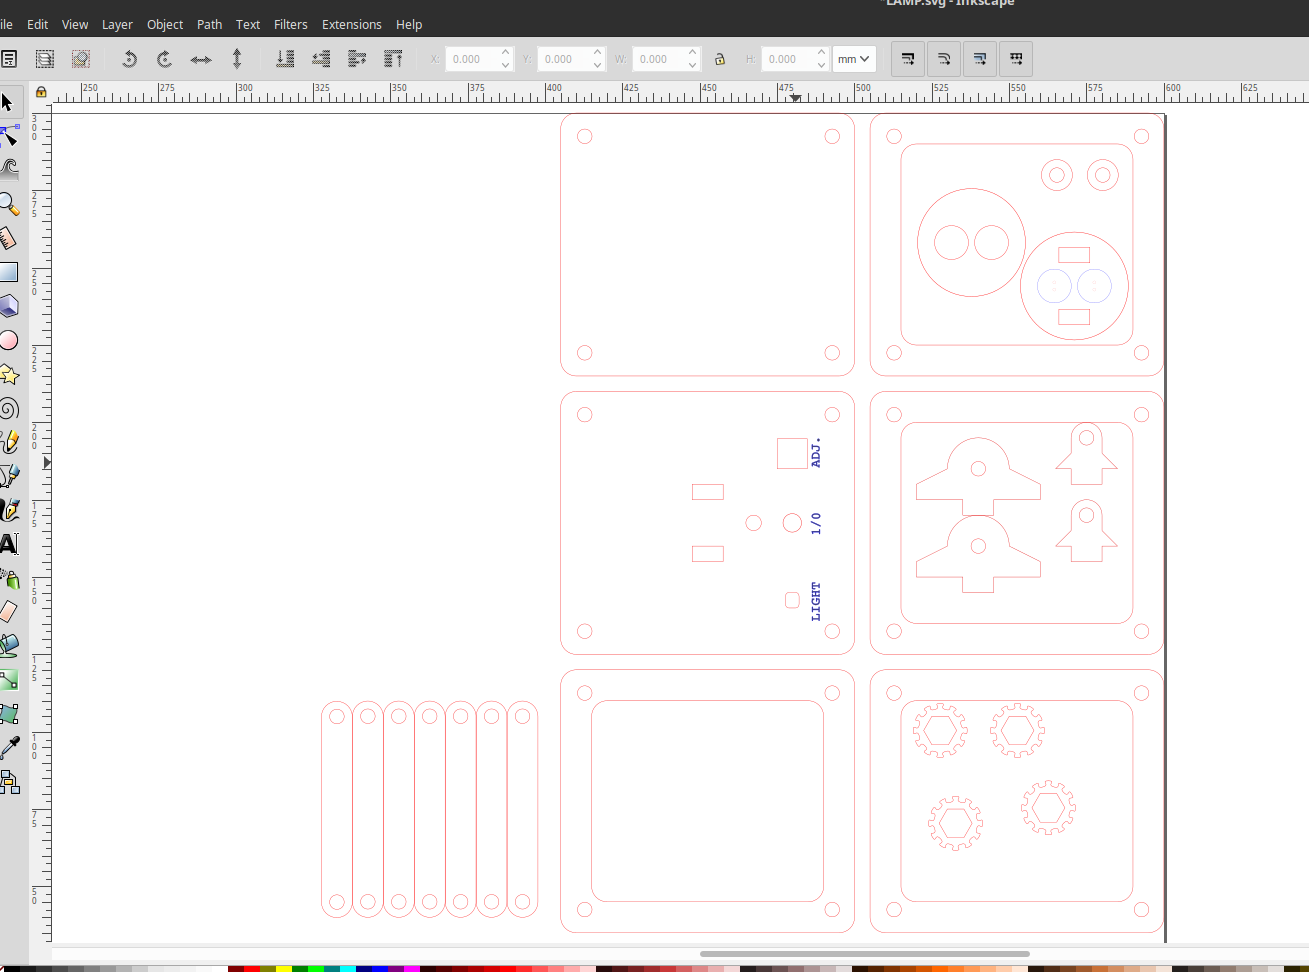
\includegraphics[width=.75\linewidth]{lampINK.png}}
\caption{Design - Inkscape}
\end{figure}

\begin{figure}[h!]
\centerline{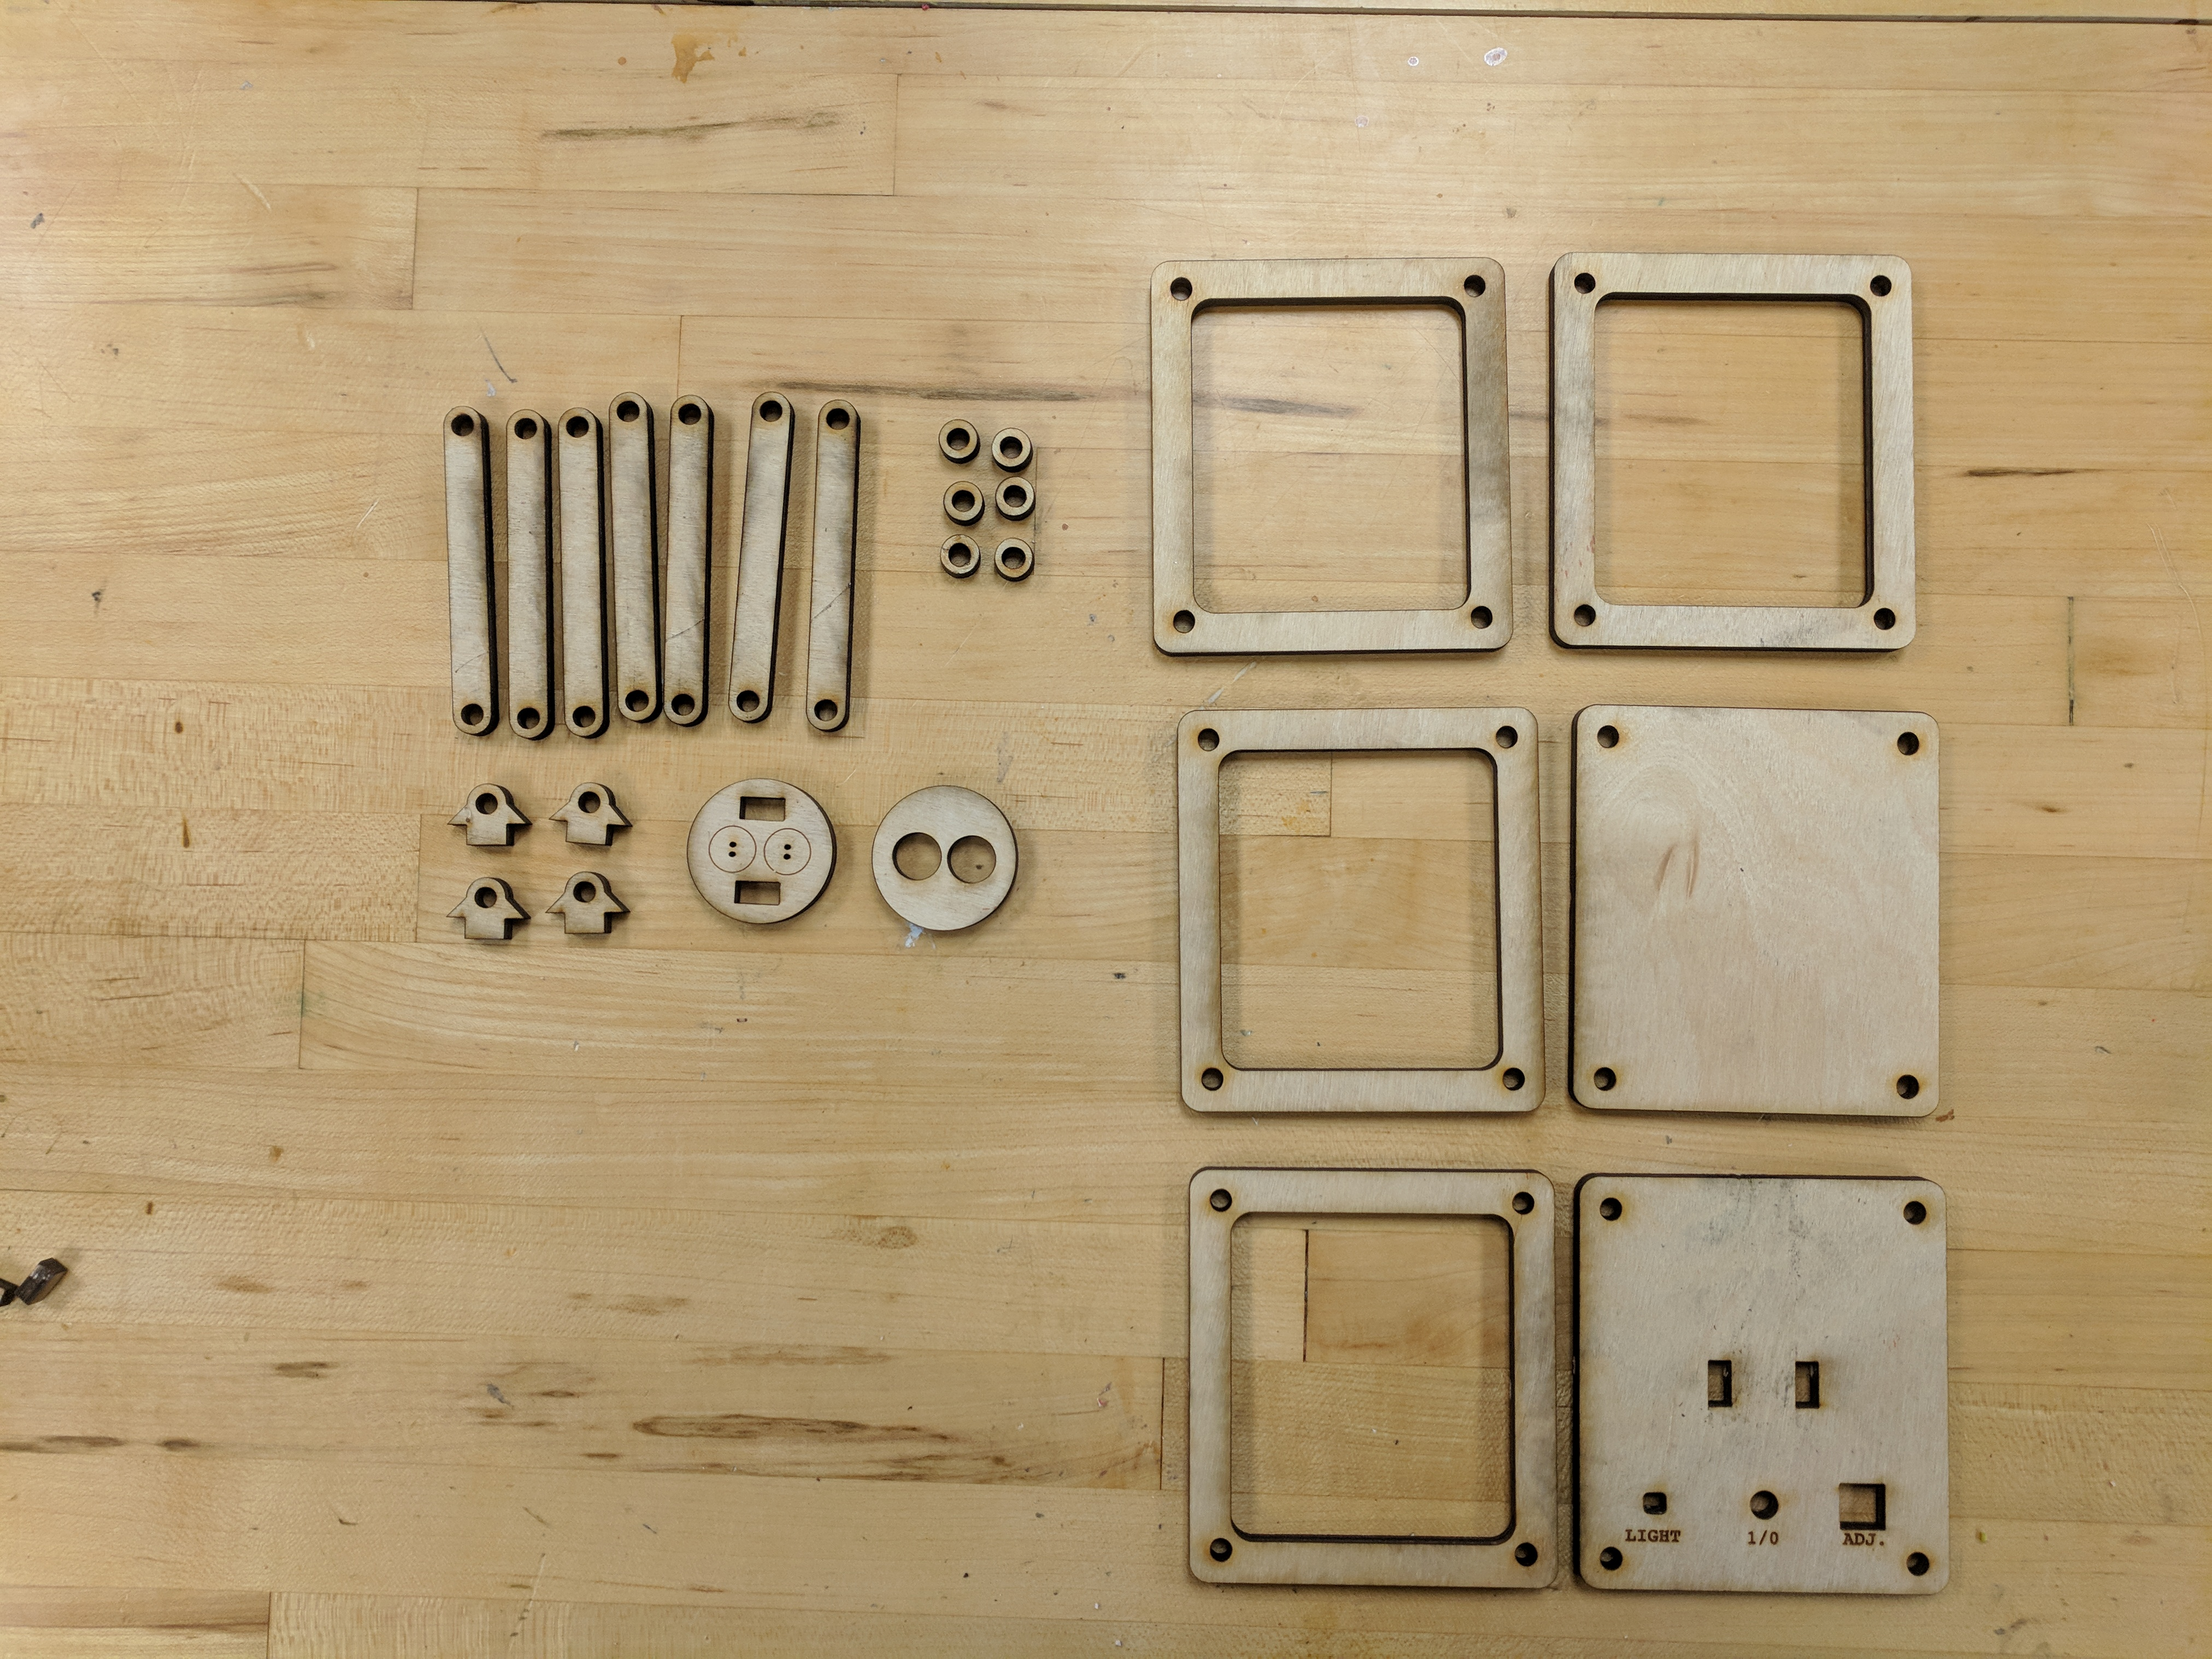
\includegraphics[width=.75\linewidth]{lamp1.jpg}}
\caption{Laser Cut - 5mm Plywood}
\end{figure}

\begin{figure}[h!]
\centerline{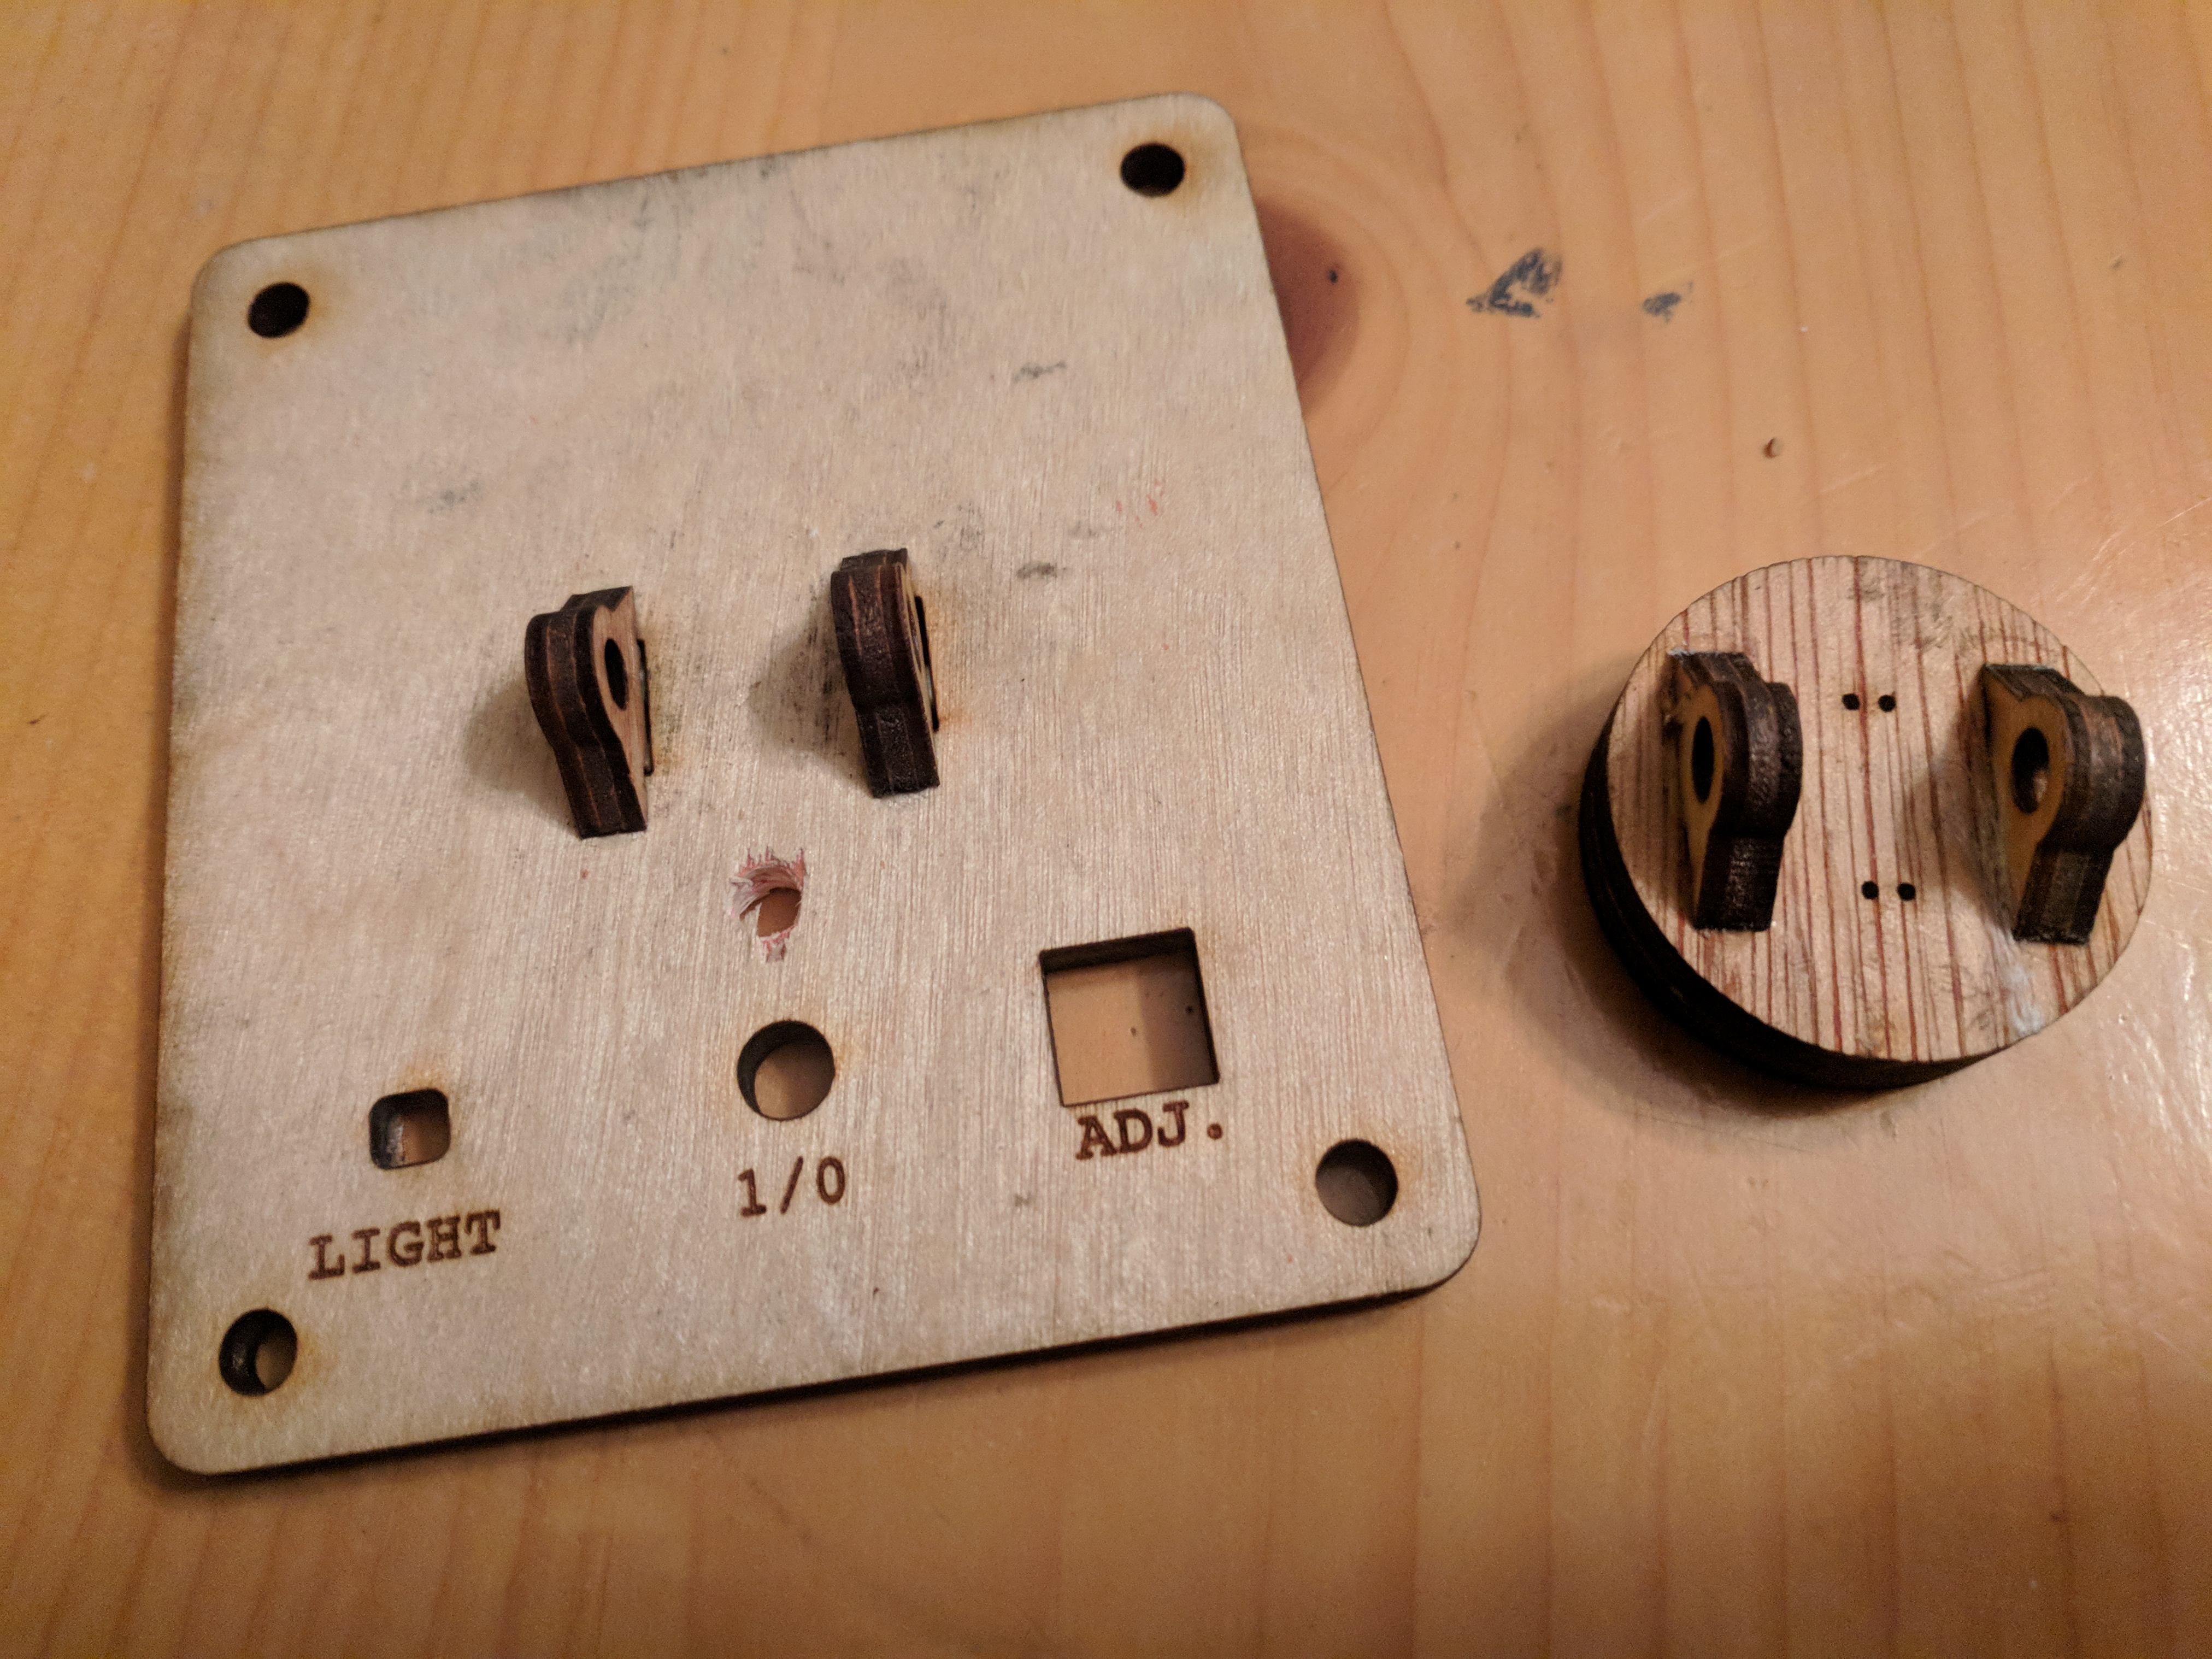
\includegraphics[width=.75\linewidth]{lamp2.jpg}}
\caption{Glue the pivot pieces to the lamp head and the top of the base}
\end{figure}

\begin{figure}[h!]
\centerline{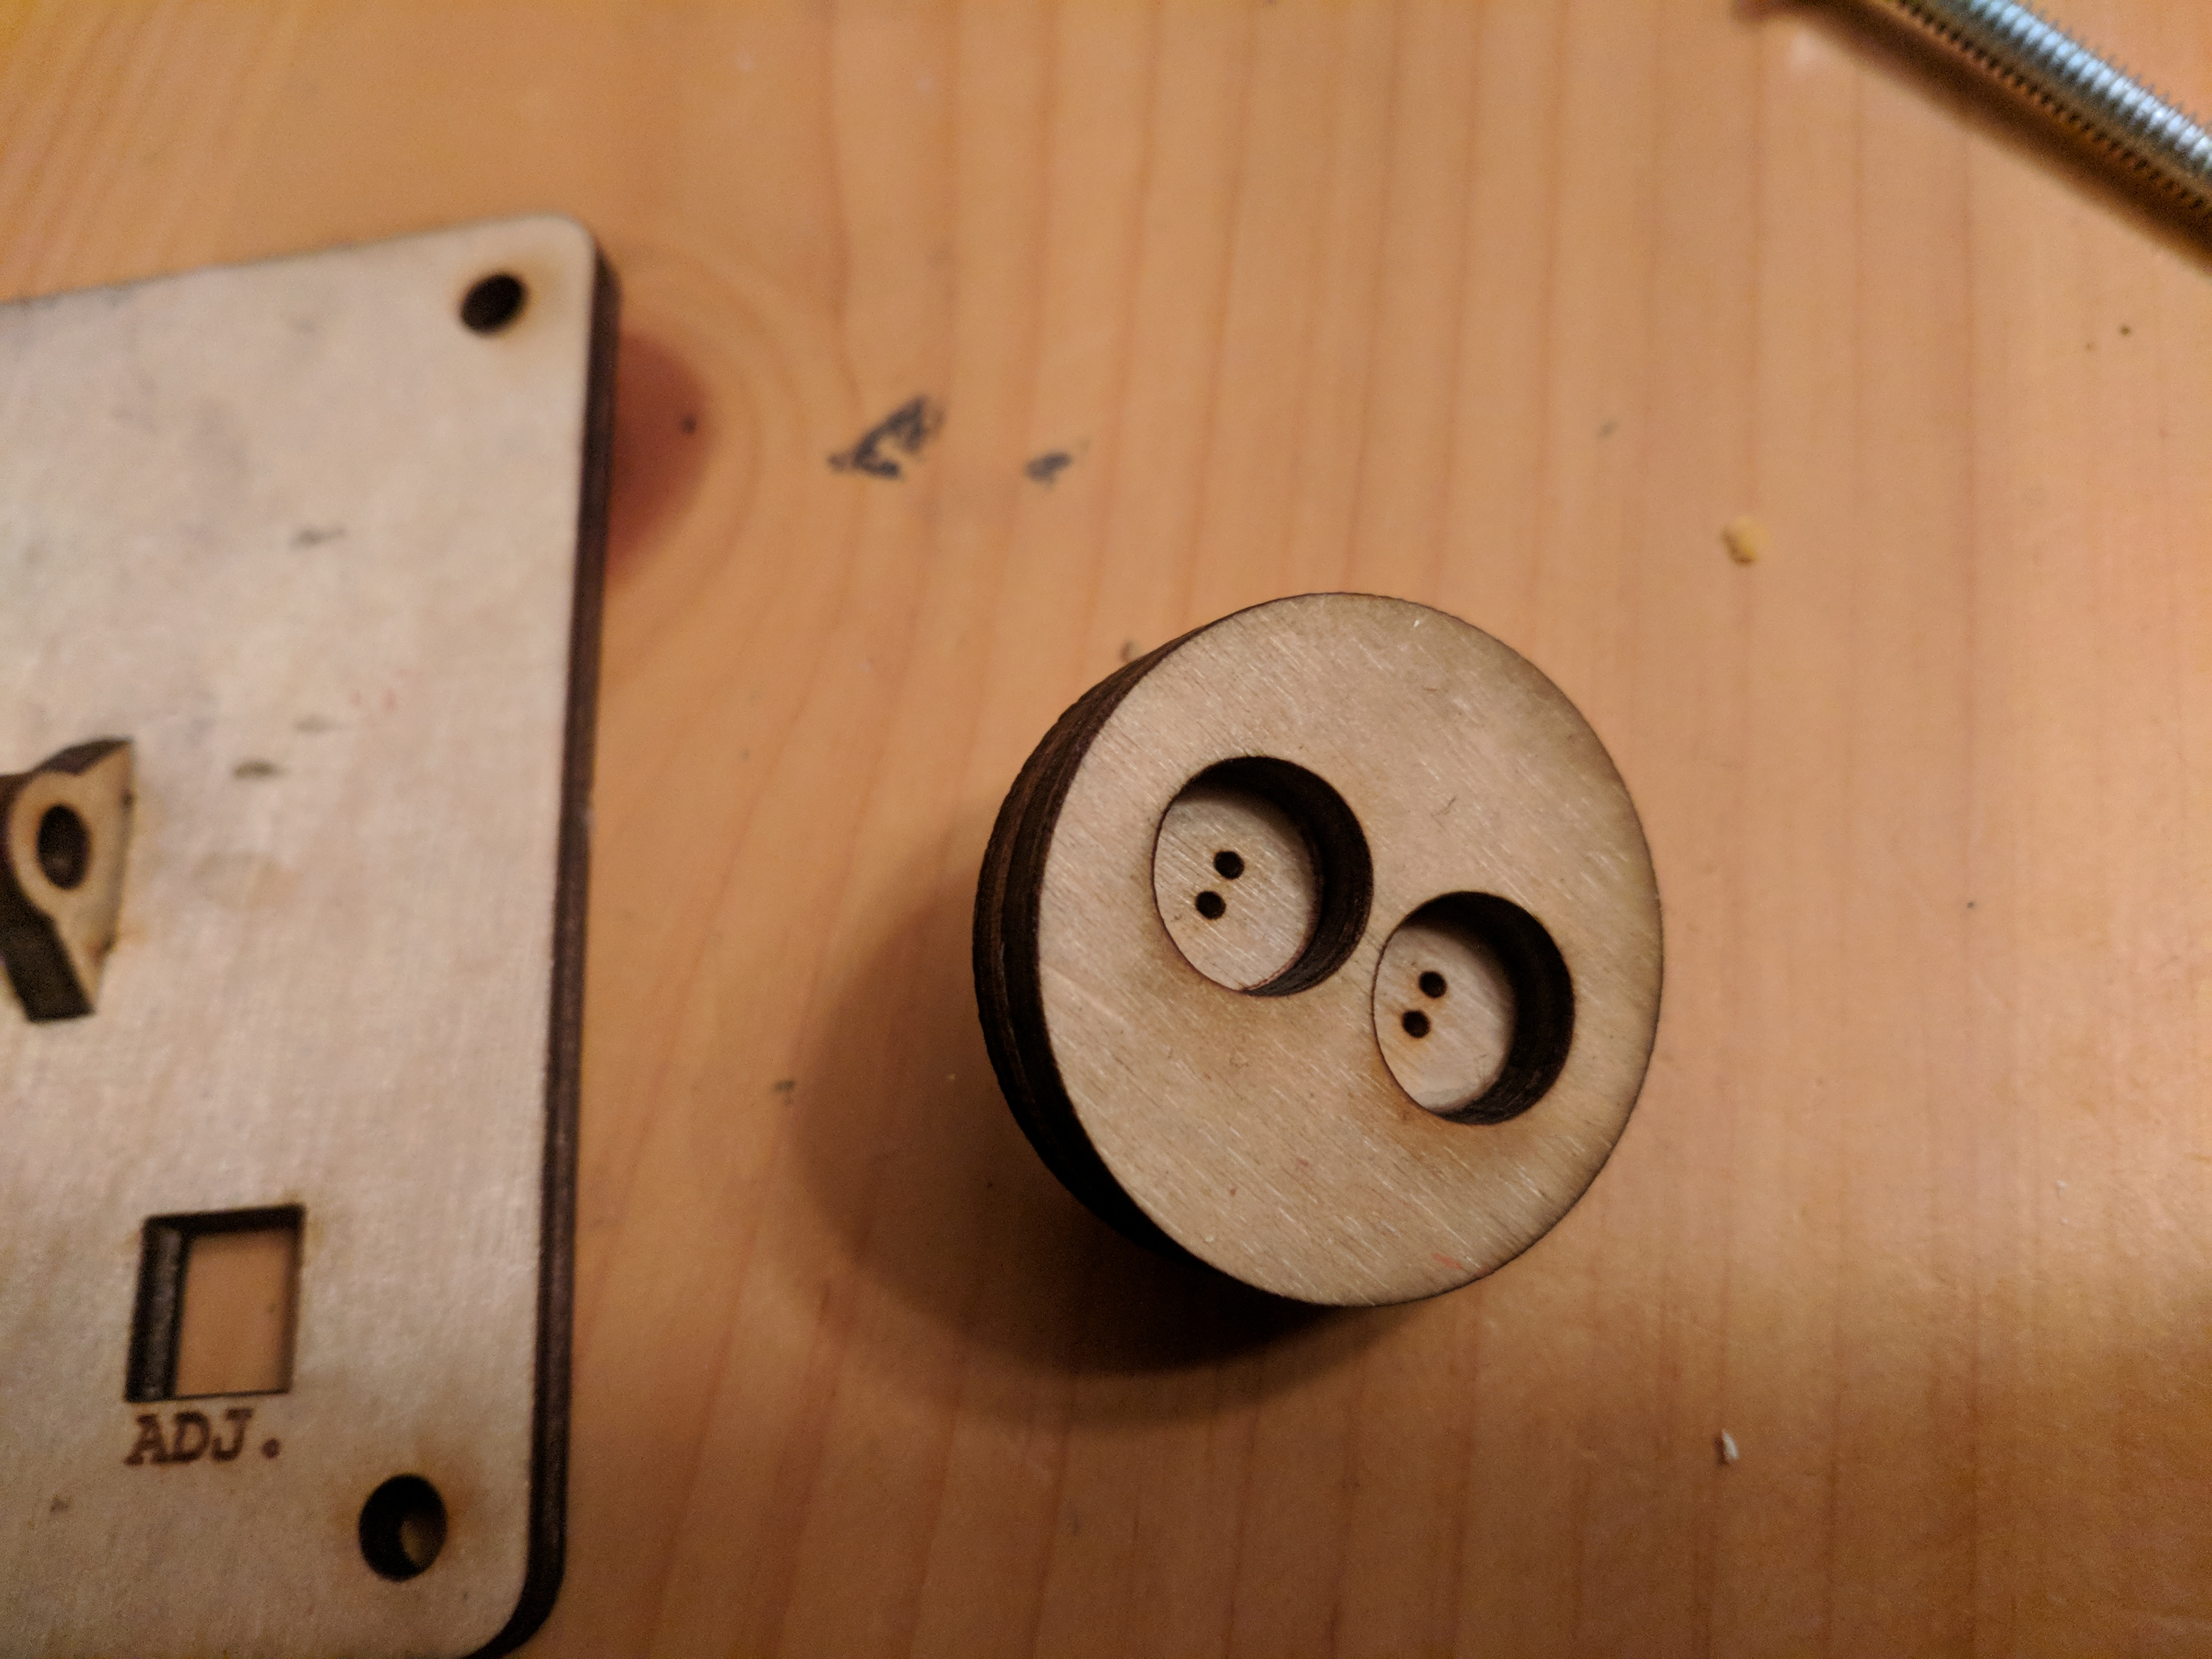
\includegraphics[width=.75\linewidth]{lamp3.jpg}}
\caption{Align and glue the two lamp head pieces together}
\end{figure}

\begin{figure}[h!]
\centerline{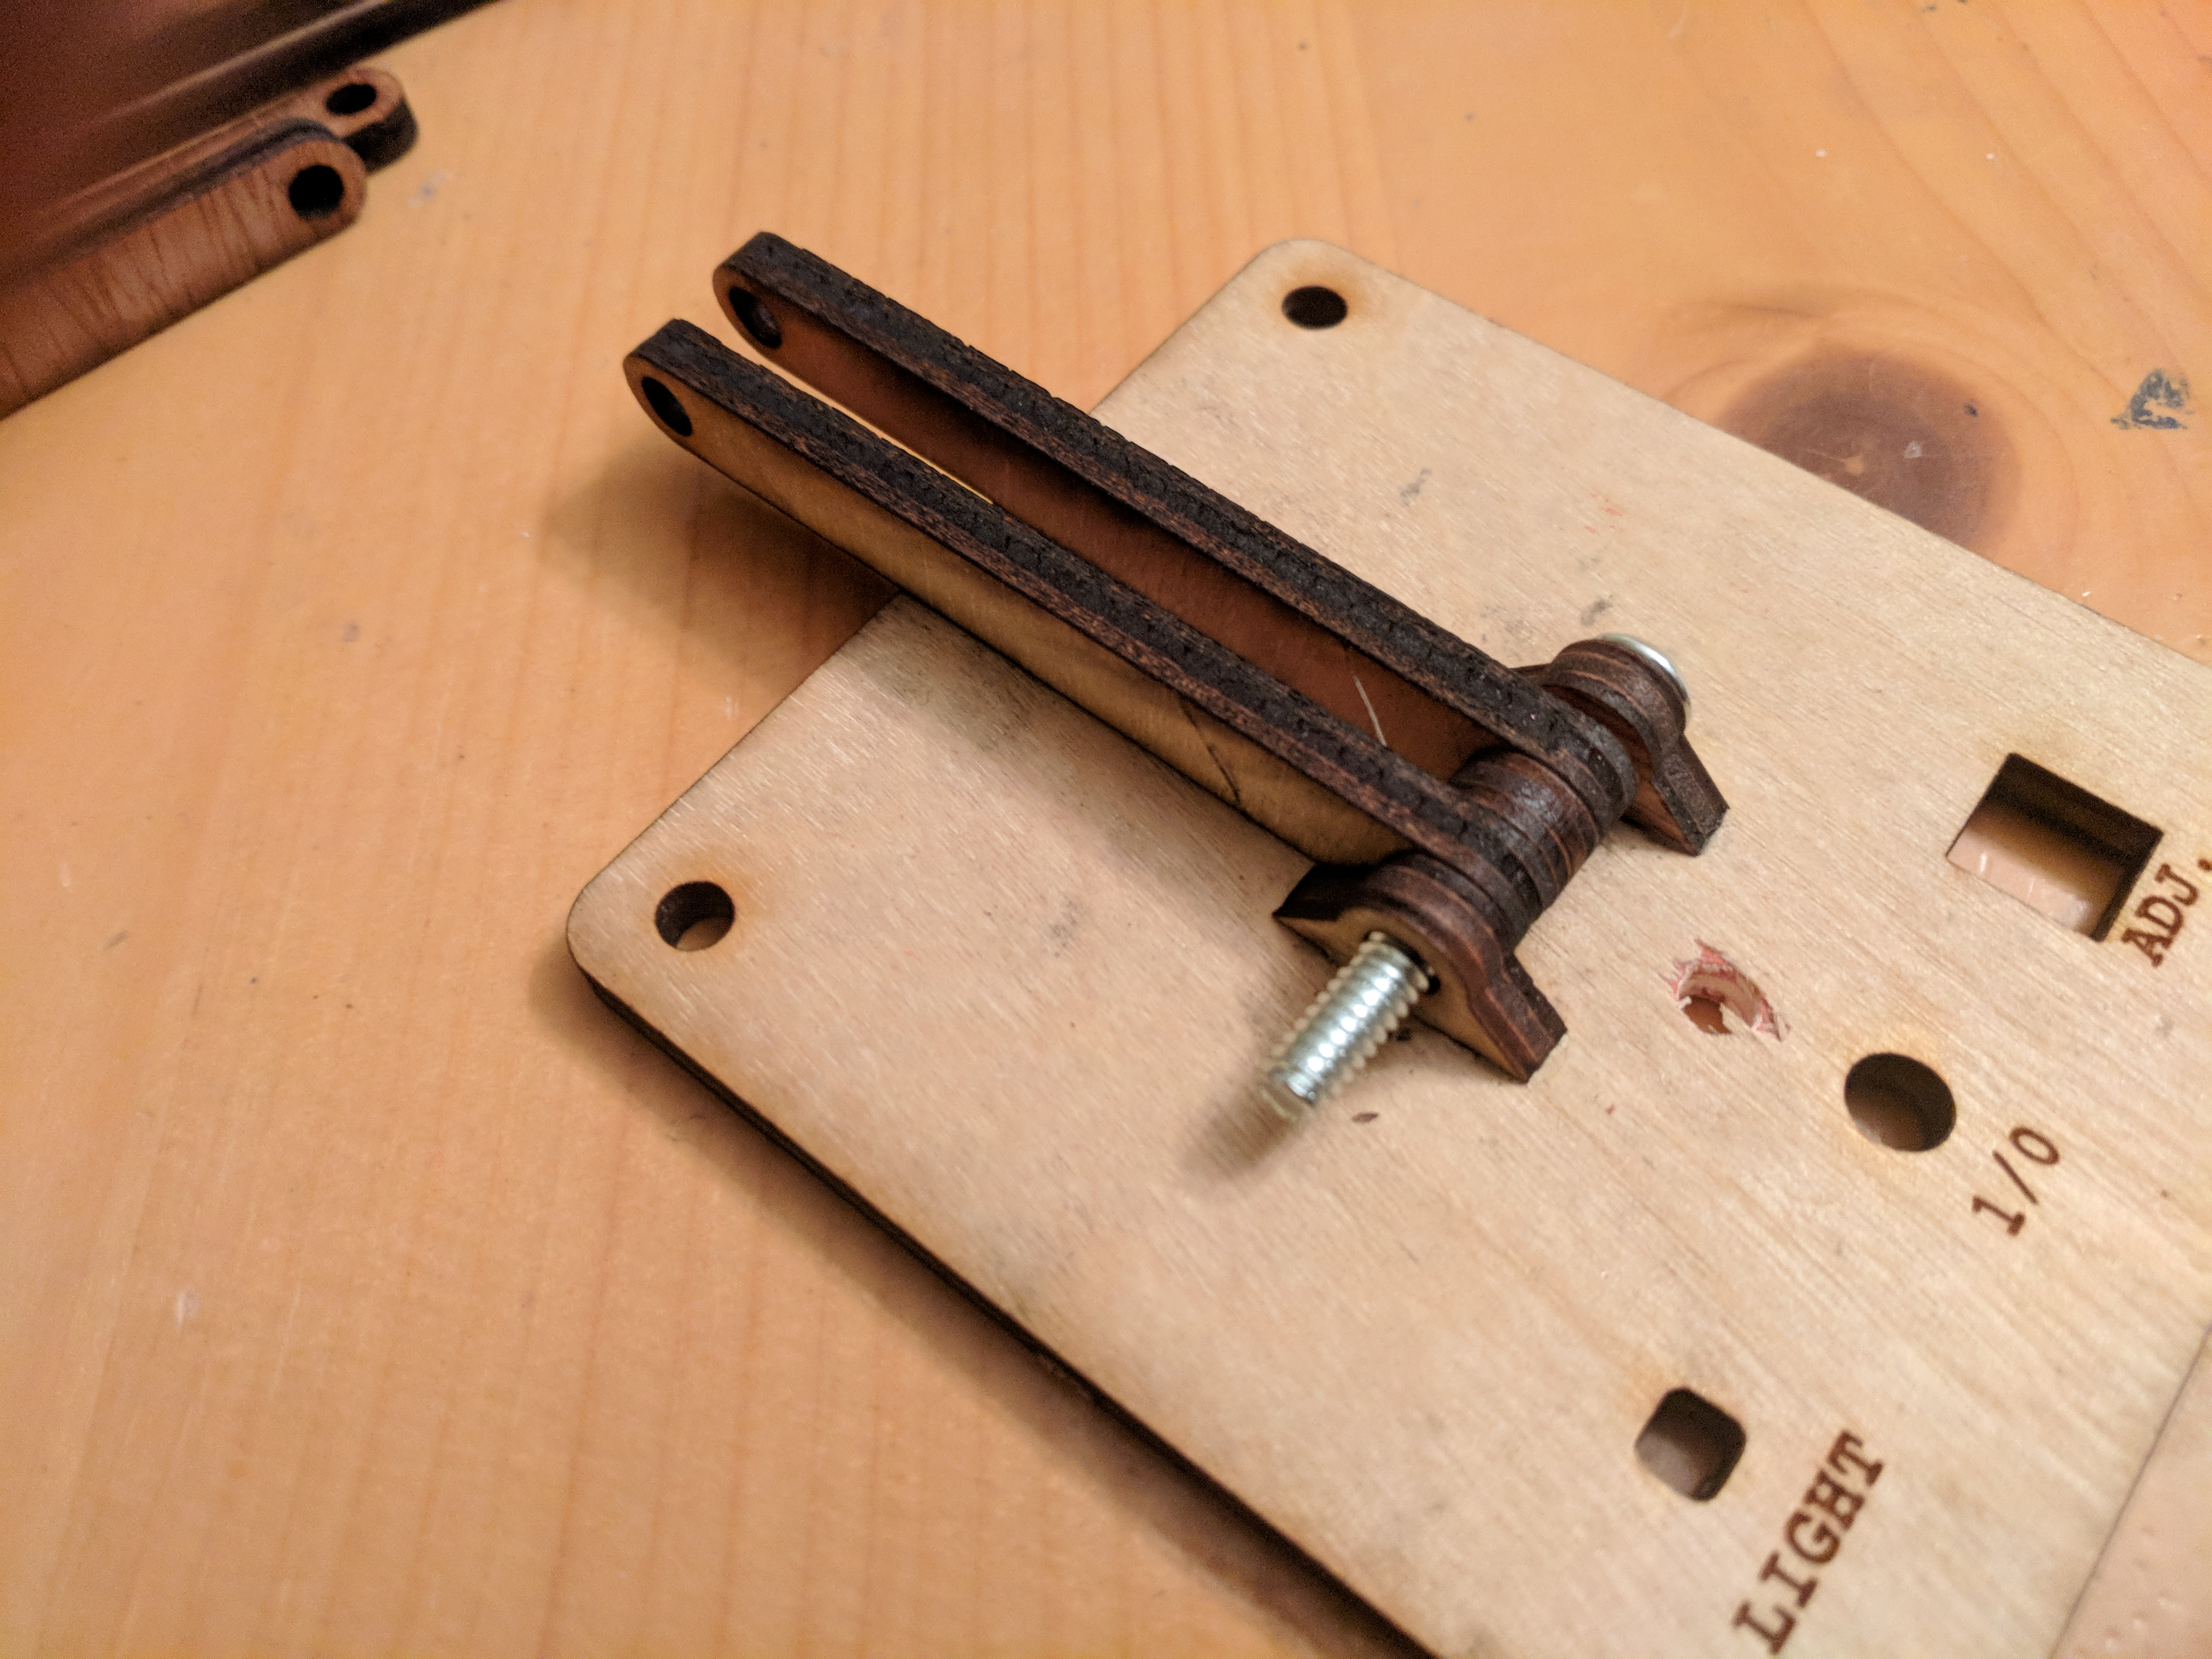
\includegraphics[width=.75\linewidth]{lamp4.jpg}}
\caption{10-24 bolt through the pivot joint on the base, add a spacer between the first two arm pieces}
\end{figure}

\begin{figure}[h!]
\centerline{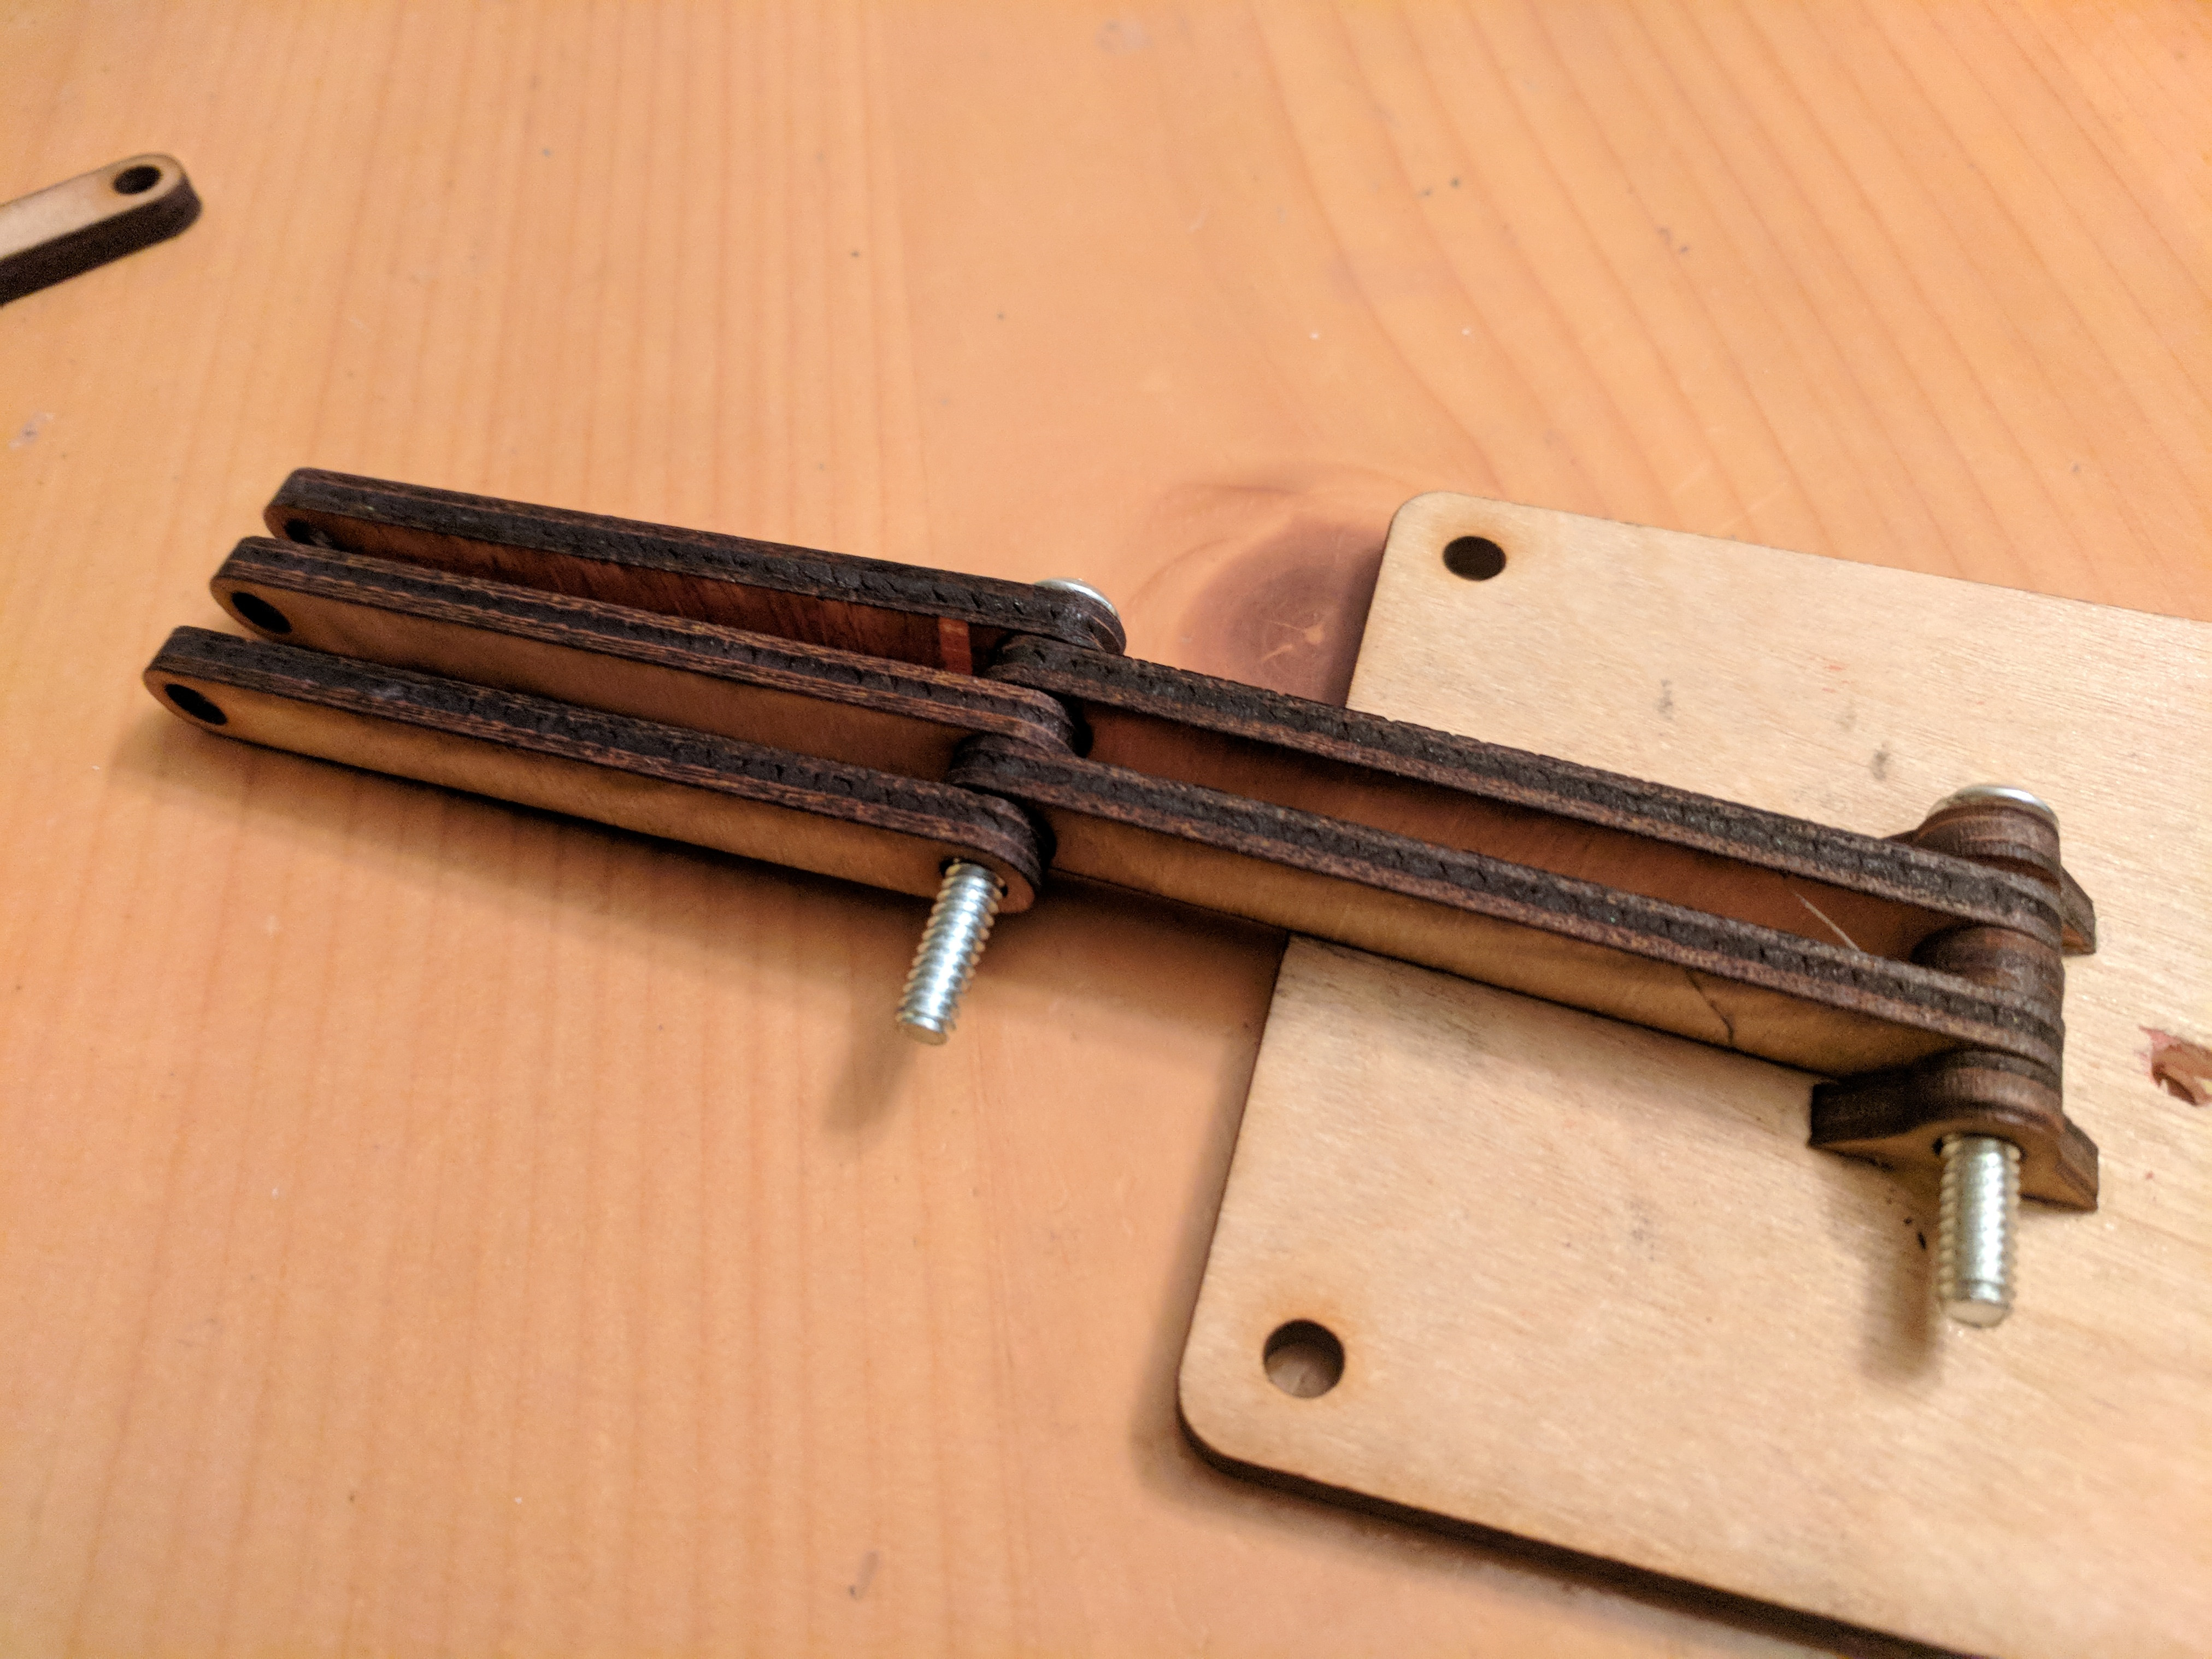
\includegraphics[width=.75\linewidth]{lamp5.jpg}}
\caption{Add three more arm pieces and place a 10-24 bolt through those 5 stacked}
\end{figure}

\begin{figure}[h!]
\centerline{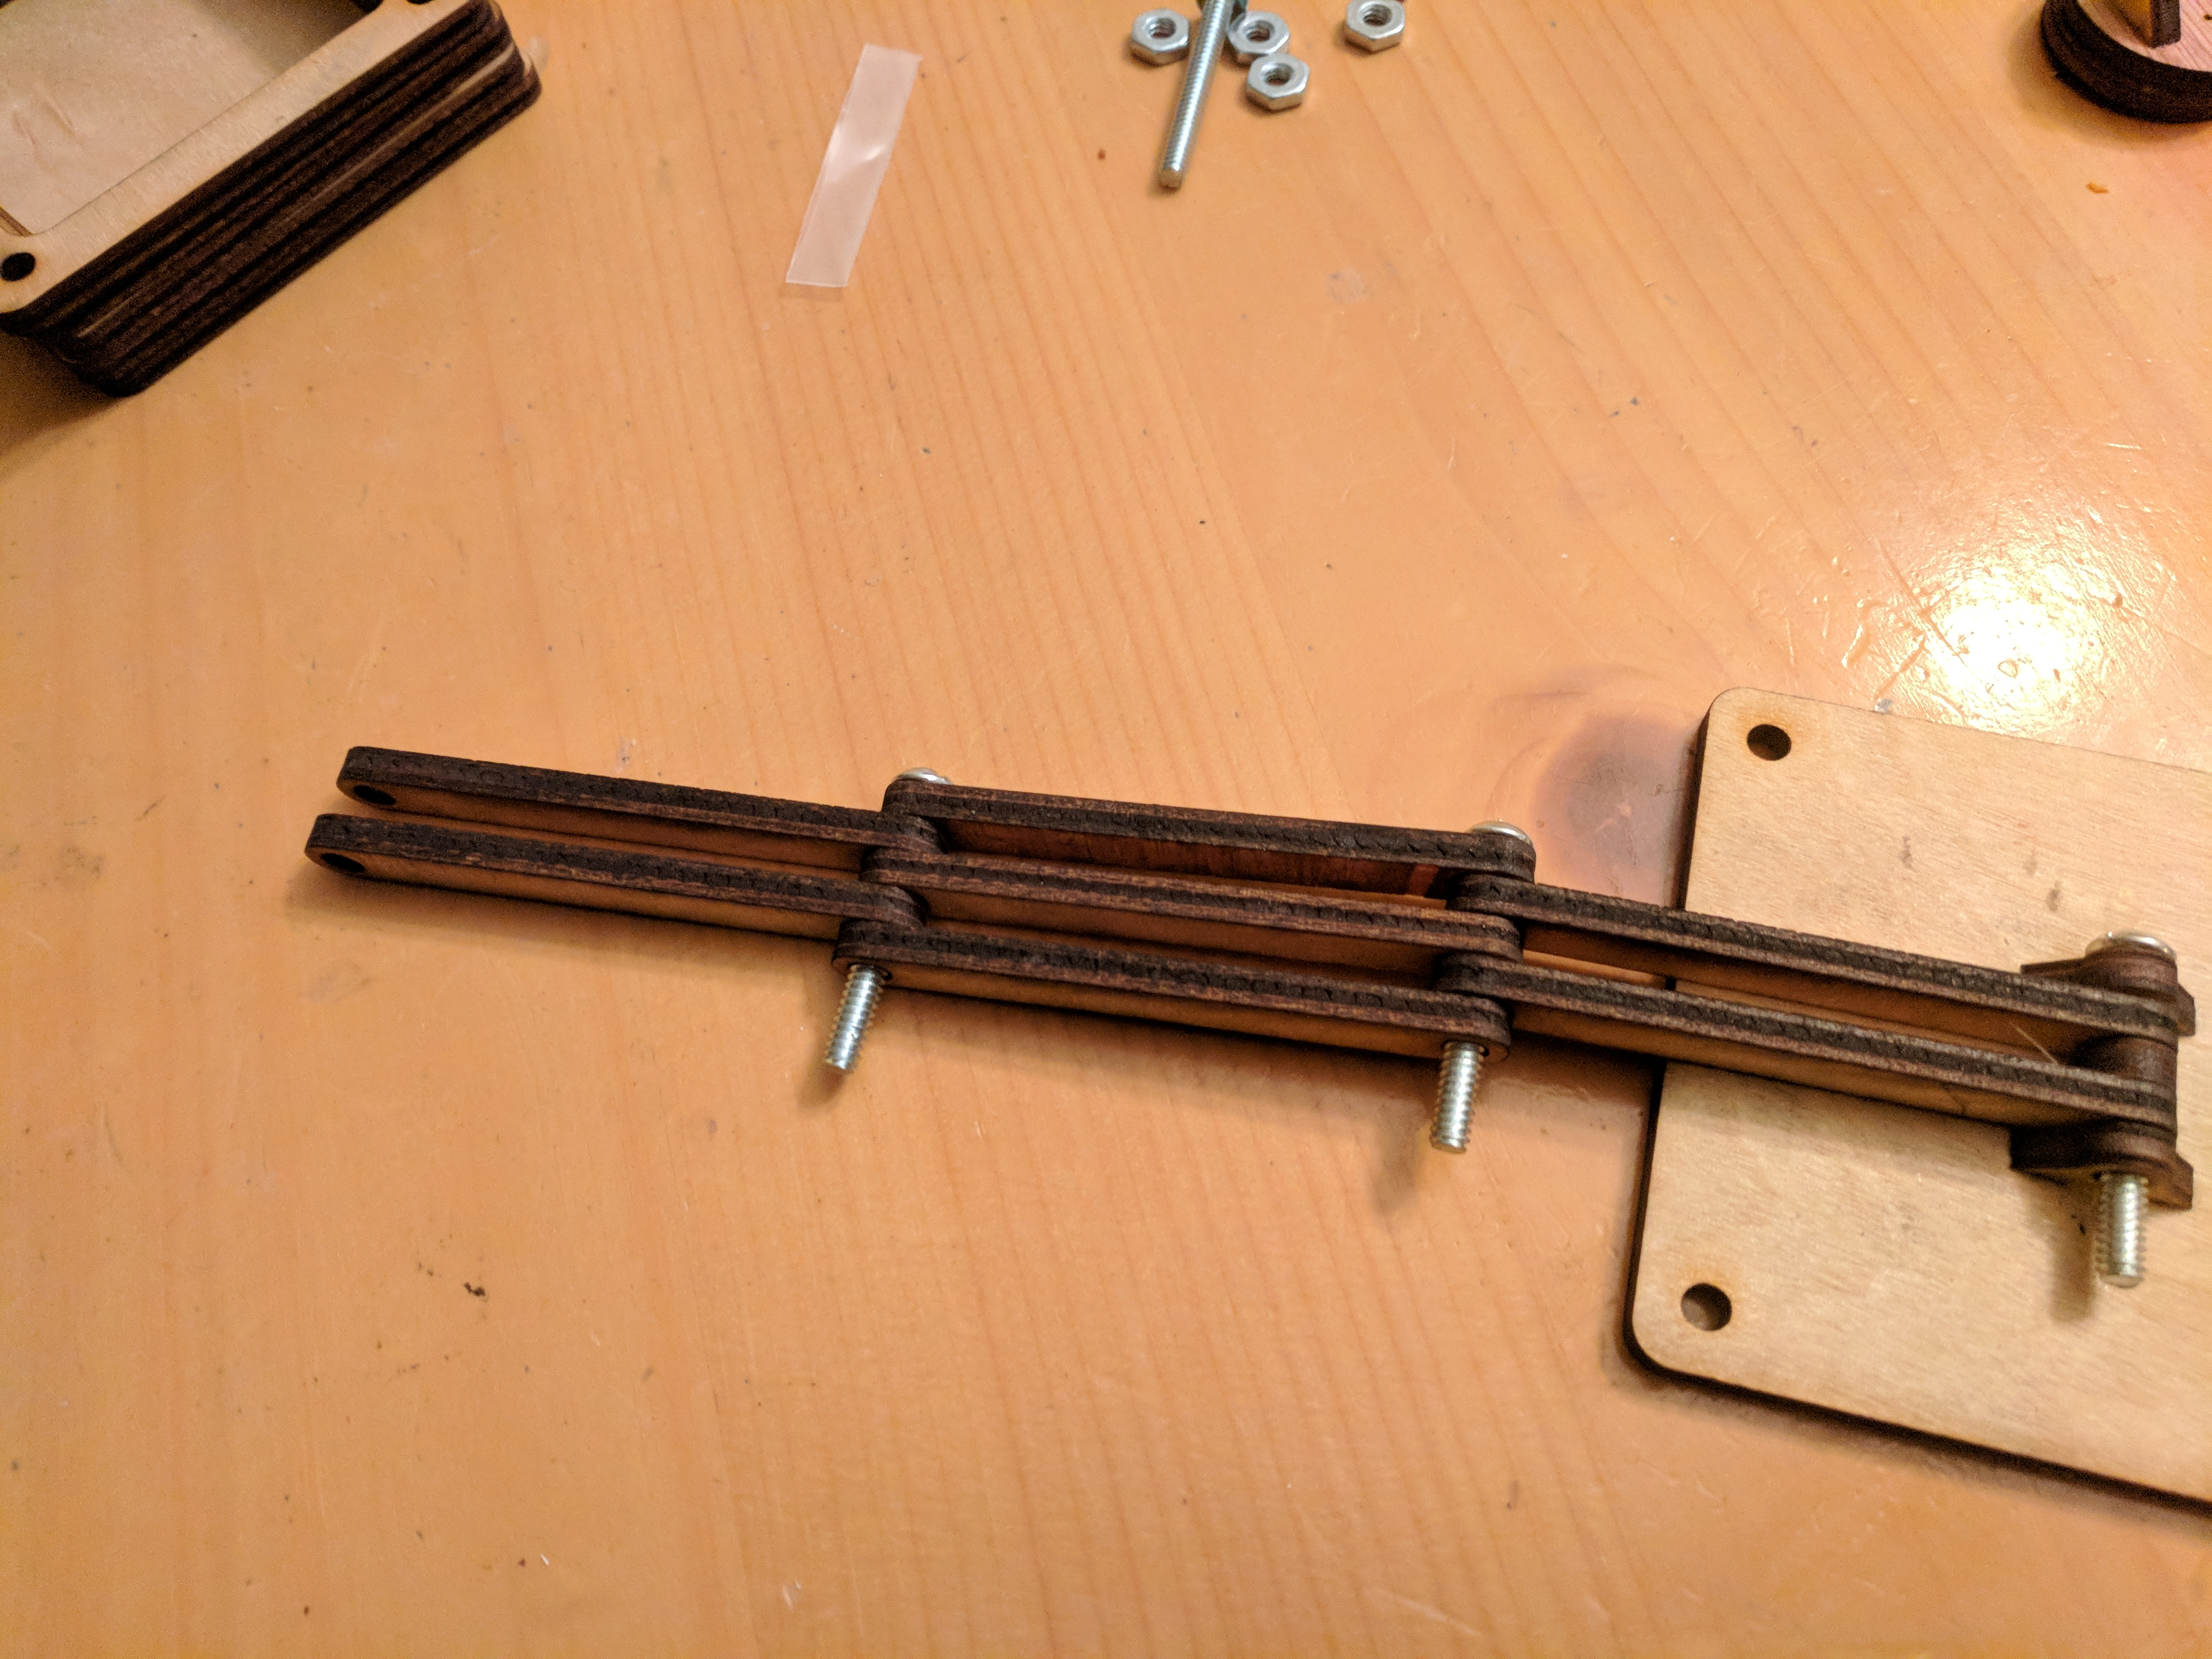
\includegraphics[width=.75\linewidth]{lamp6.jpg}}
\caption{Repeat the above process with two more arm pieces and another bolt}
\end{figure}

\begin{figure}[h!]
\centerline{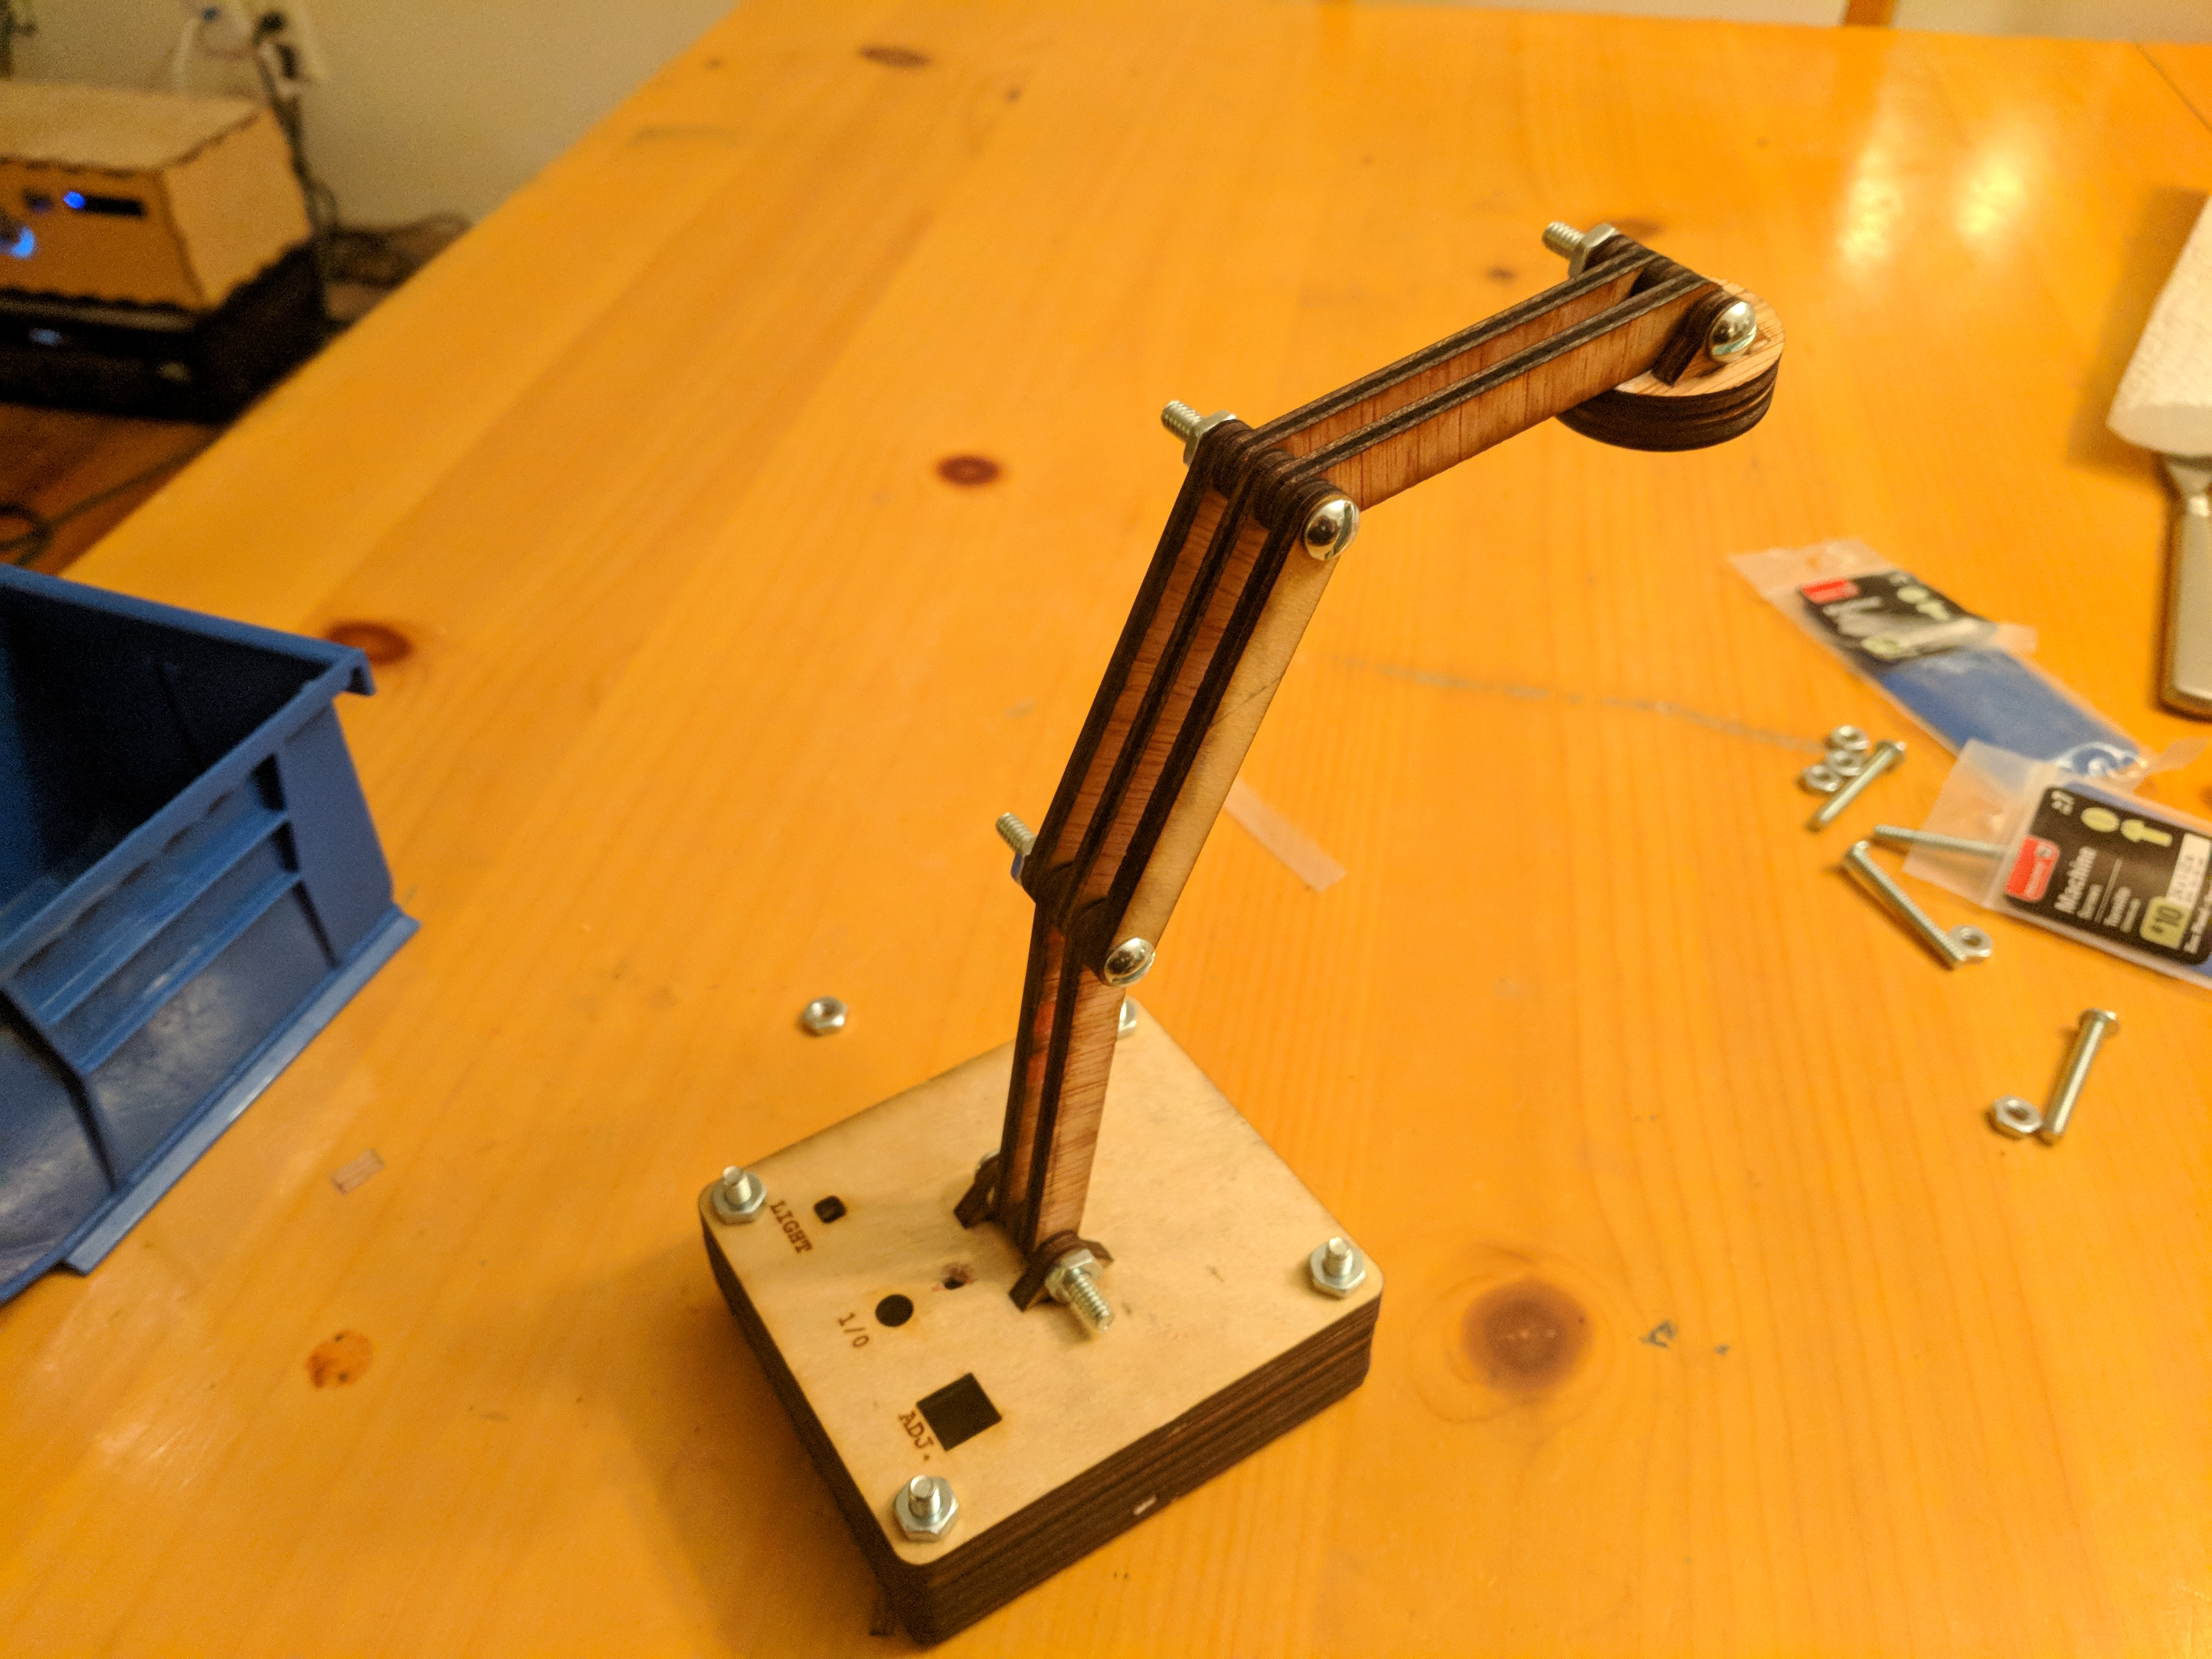
\includegraphics[width=.75\linewidth]{lamp7.jpg}}
\caption{Connect the lamp head to the last arm and include another spacer}
\end{figure}

\begin{figure}[h!]
\centerline{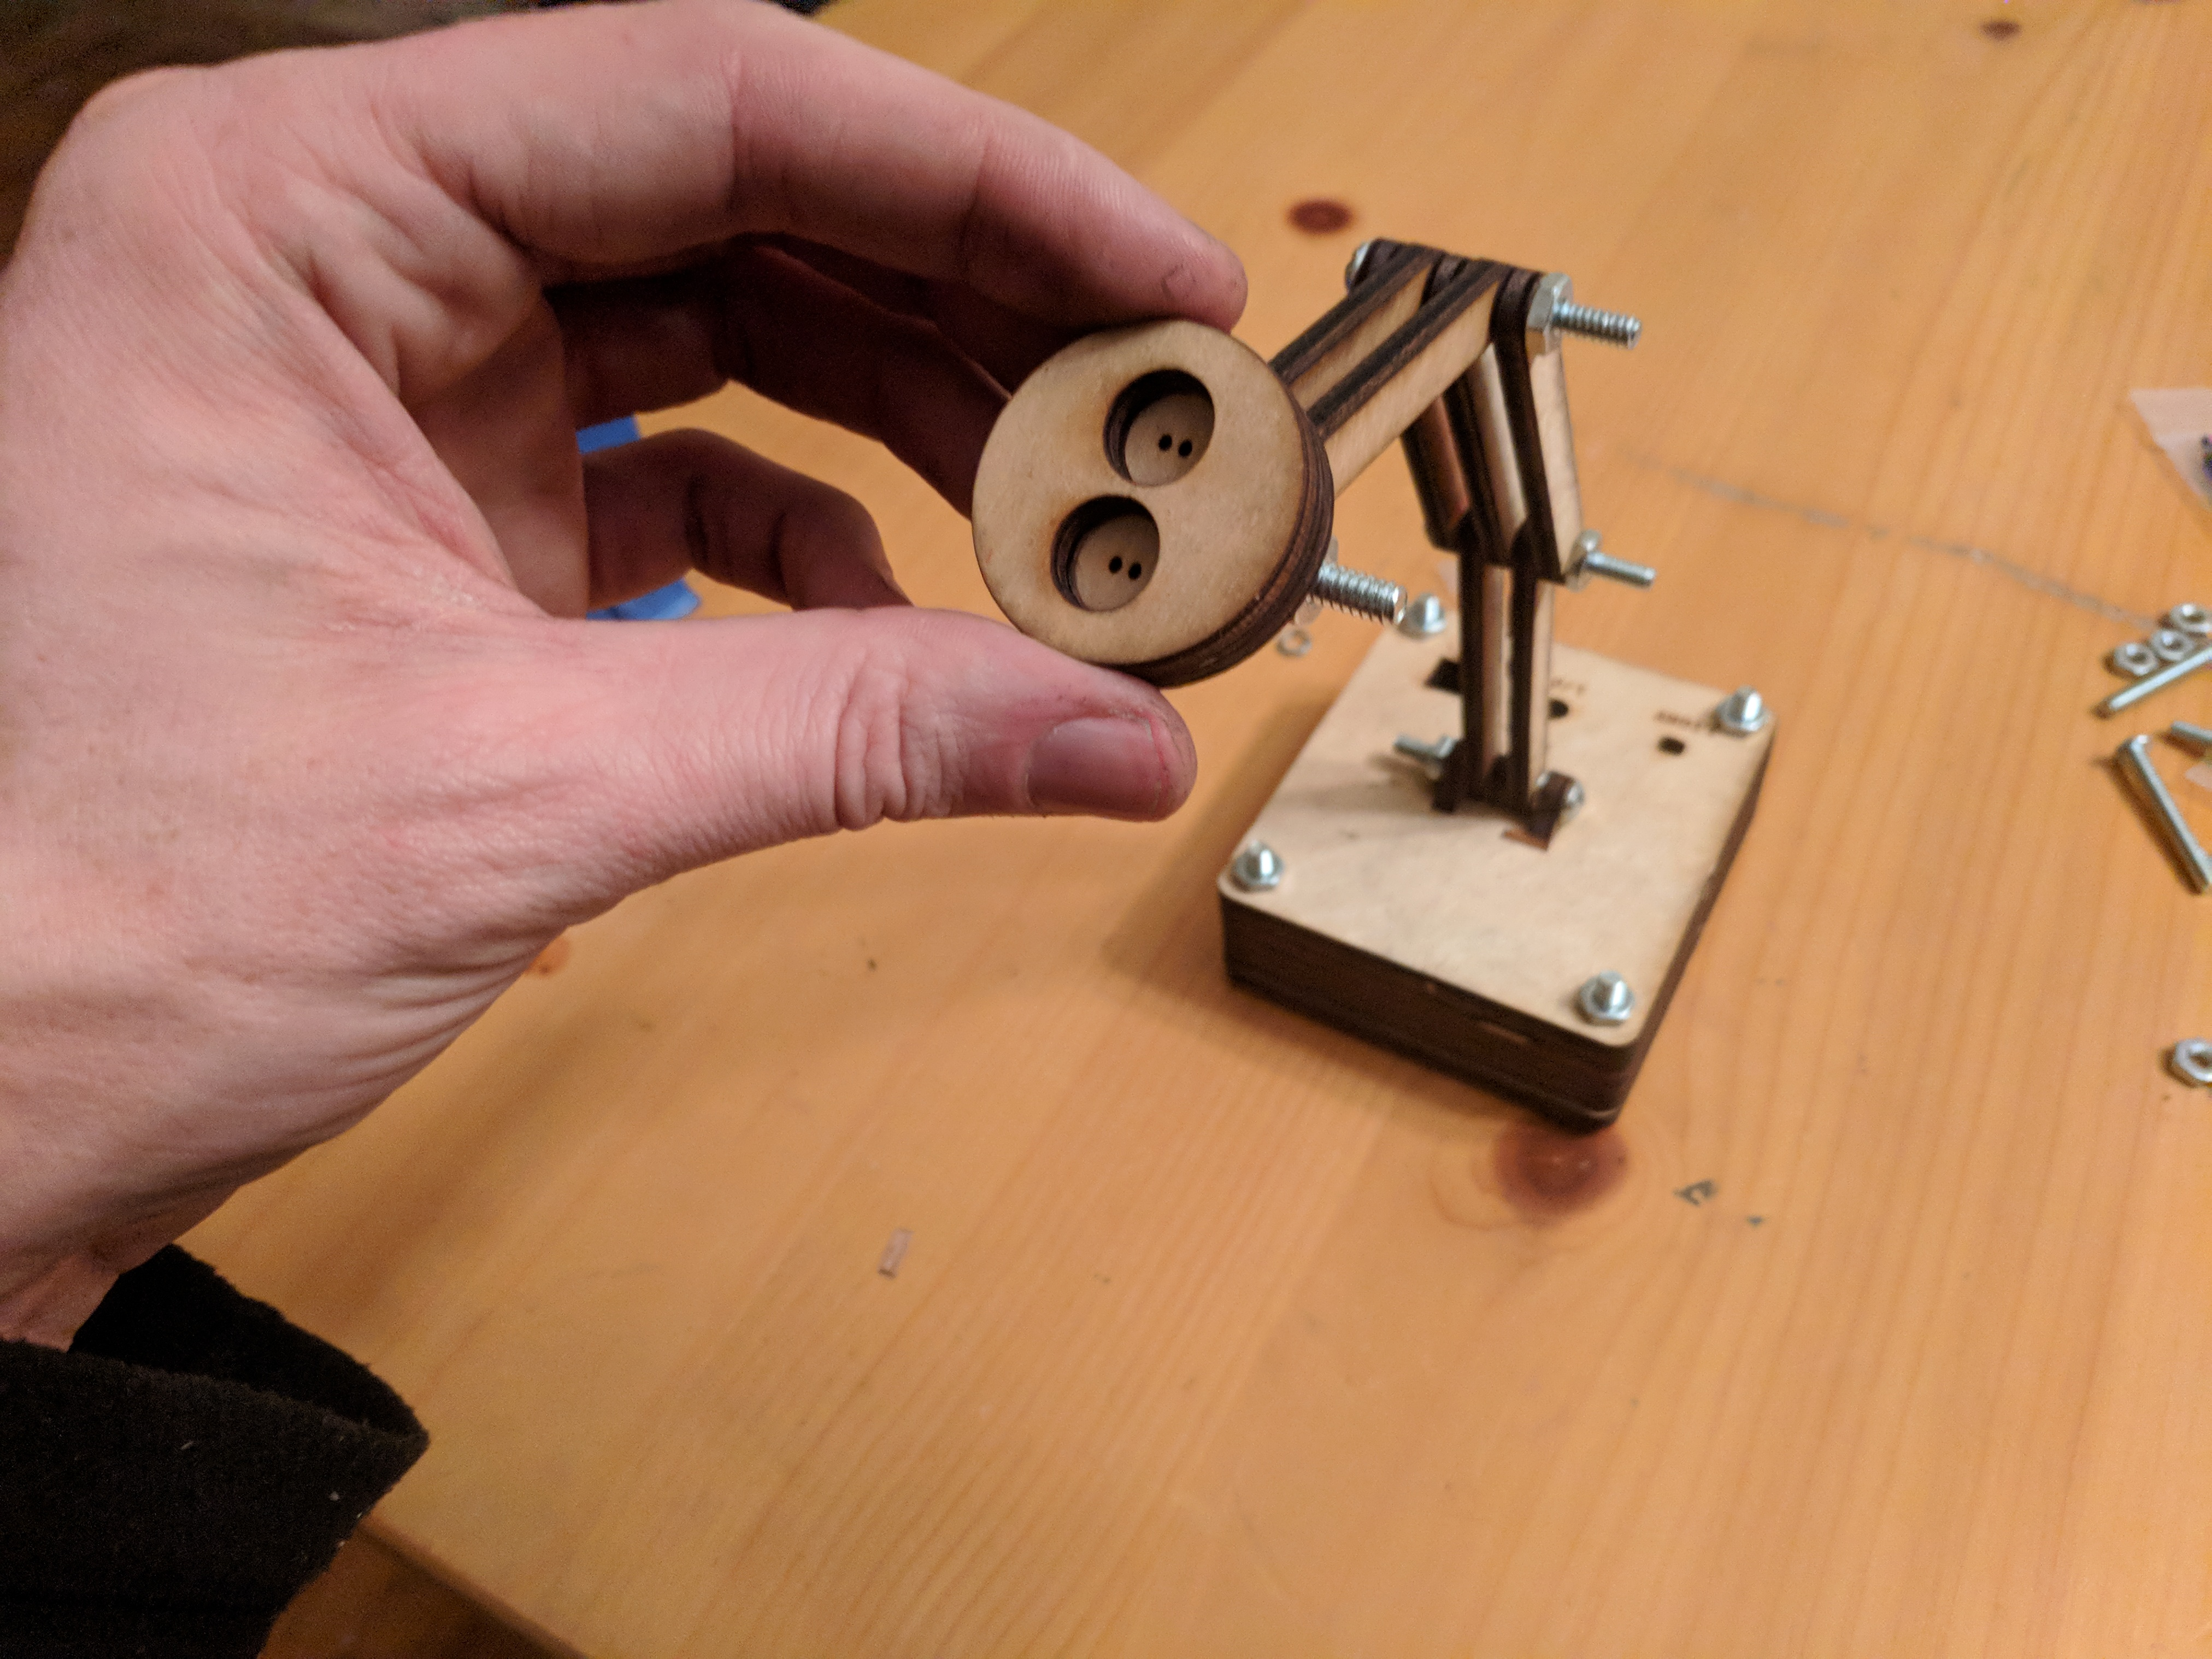
\includegraphics[width=.75\linewidth]{lamp8.jpg}}
\caption{Another view of the lamp being put together - the base is stacked with the solid pieces on the top and bottom}
\end{figure}

\begin{figure}[h!]
\centerline{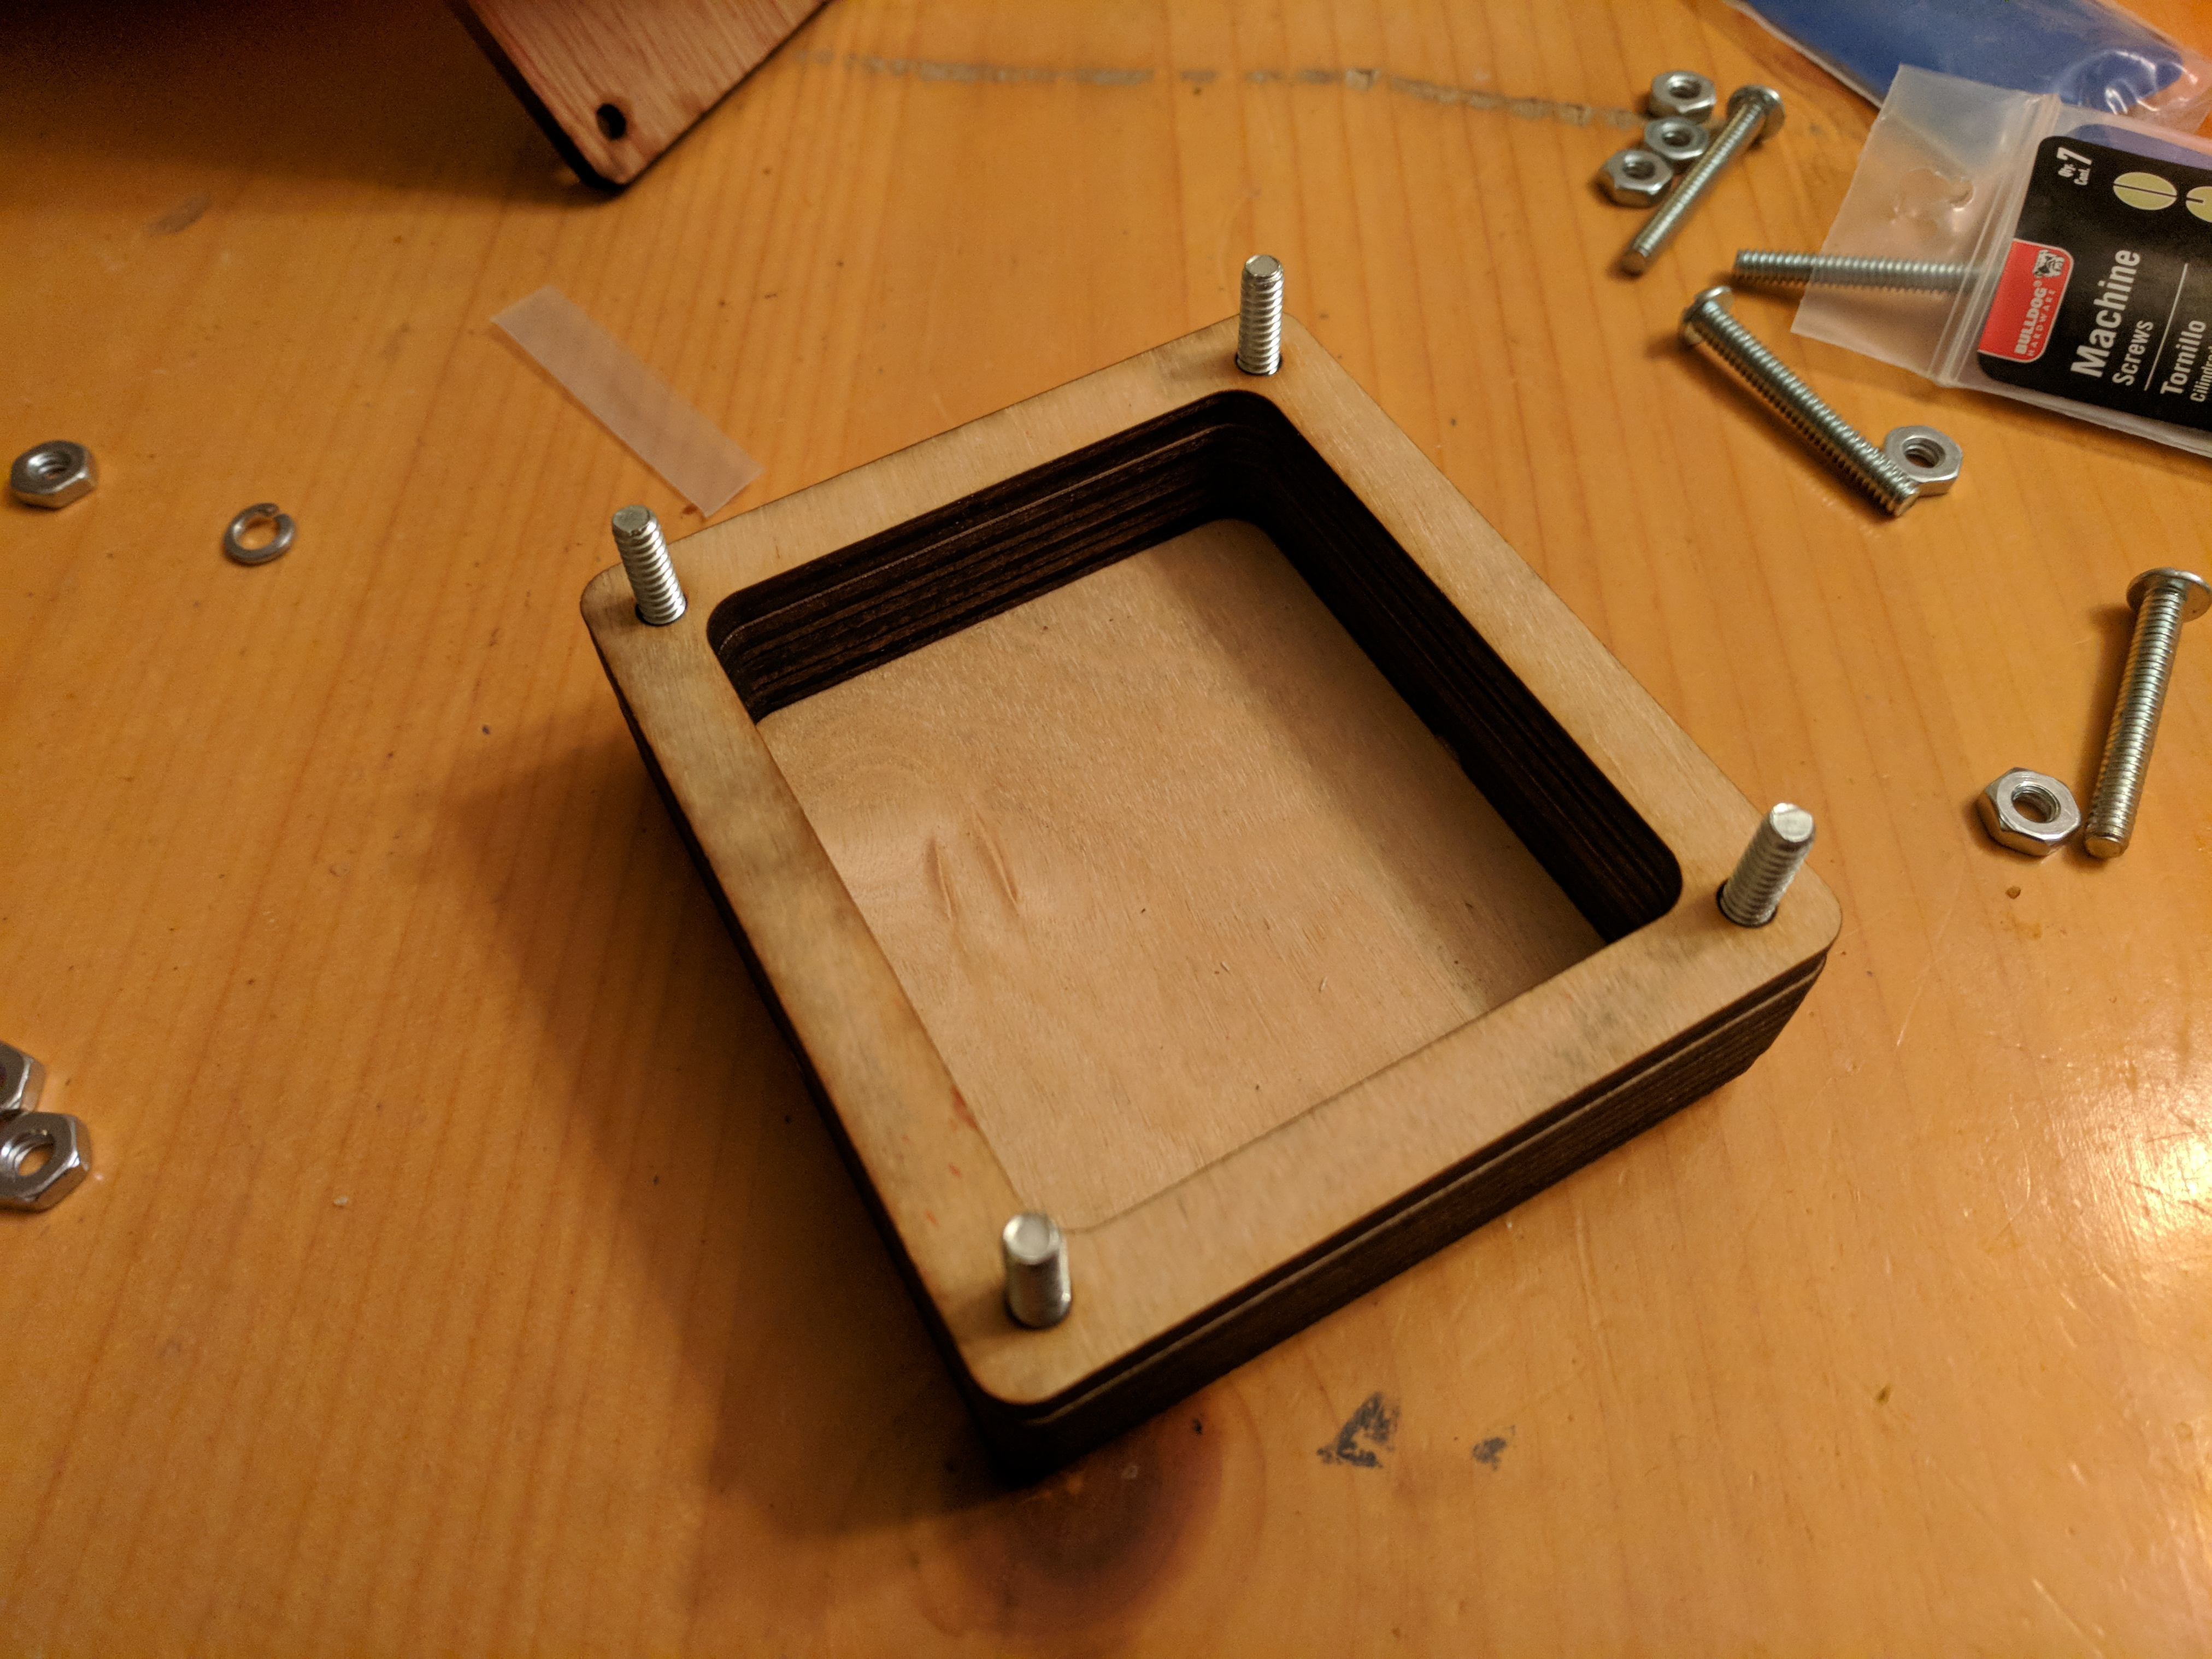
\includegraphics[width=.75\linewidth]{lamp9.jpg}}
\caption{Here is the inside of the base to hold the electronics and the battery}
\end{figure}

\begin{figure}[h!]
\centerline{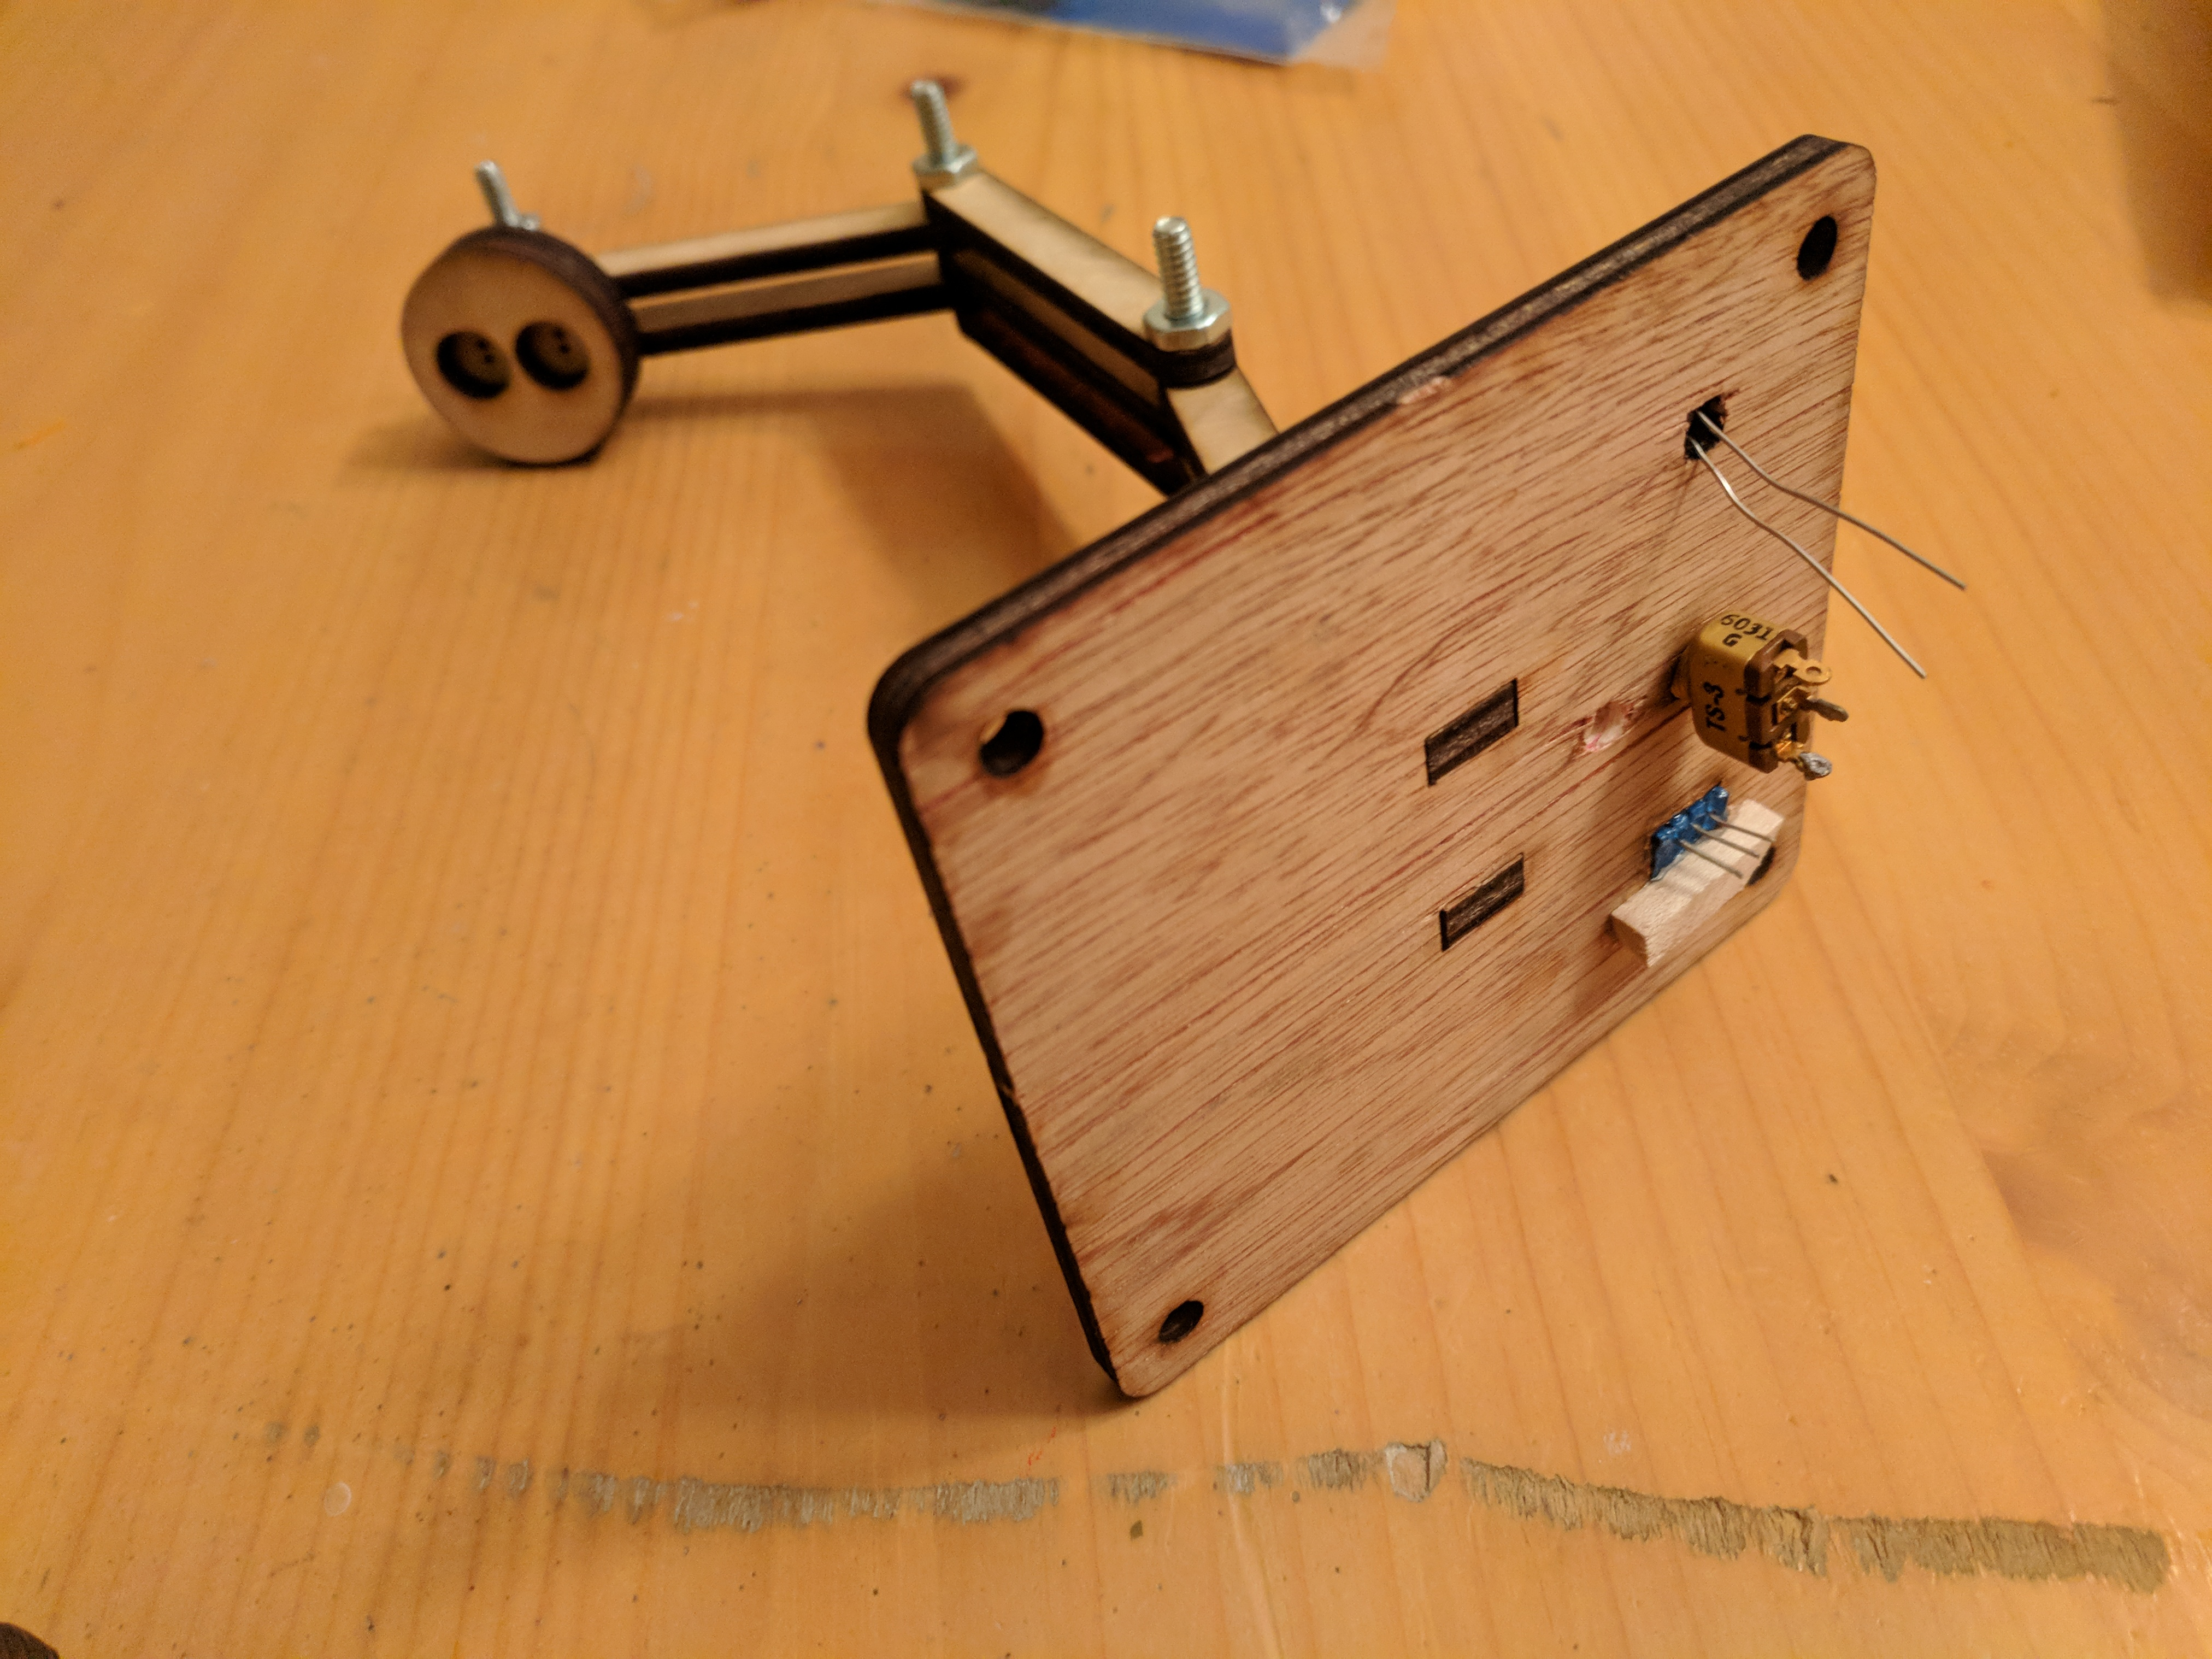
\includegraphics[width=.75\linewidth]{lamp10.jpg}}
\caption{All of the electronic components are placed in the top of the base, a small strip is glued underneath the trimmer pot to keep it in place}
\end{figure}

\begin{figure}[h!]
\centerline{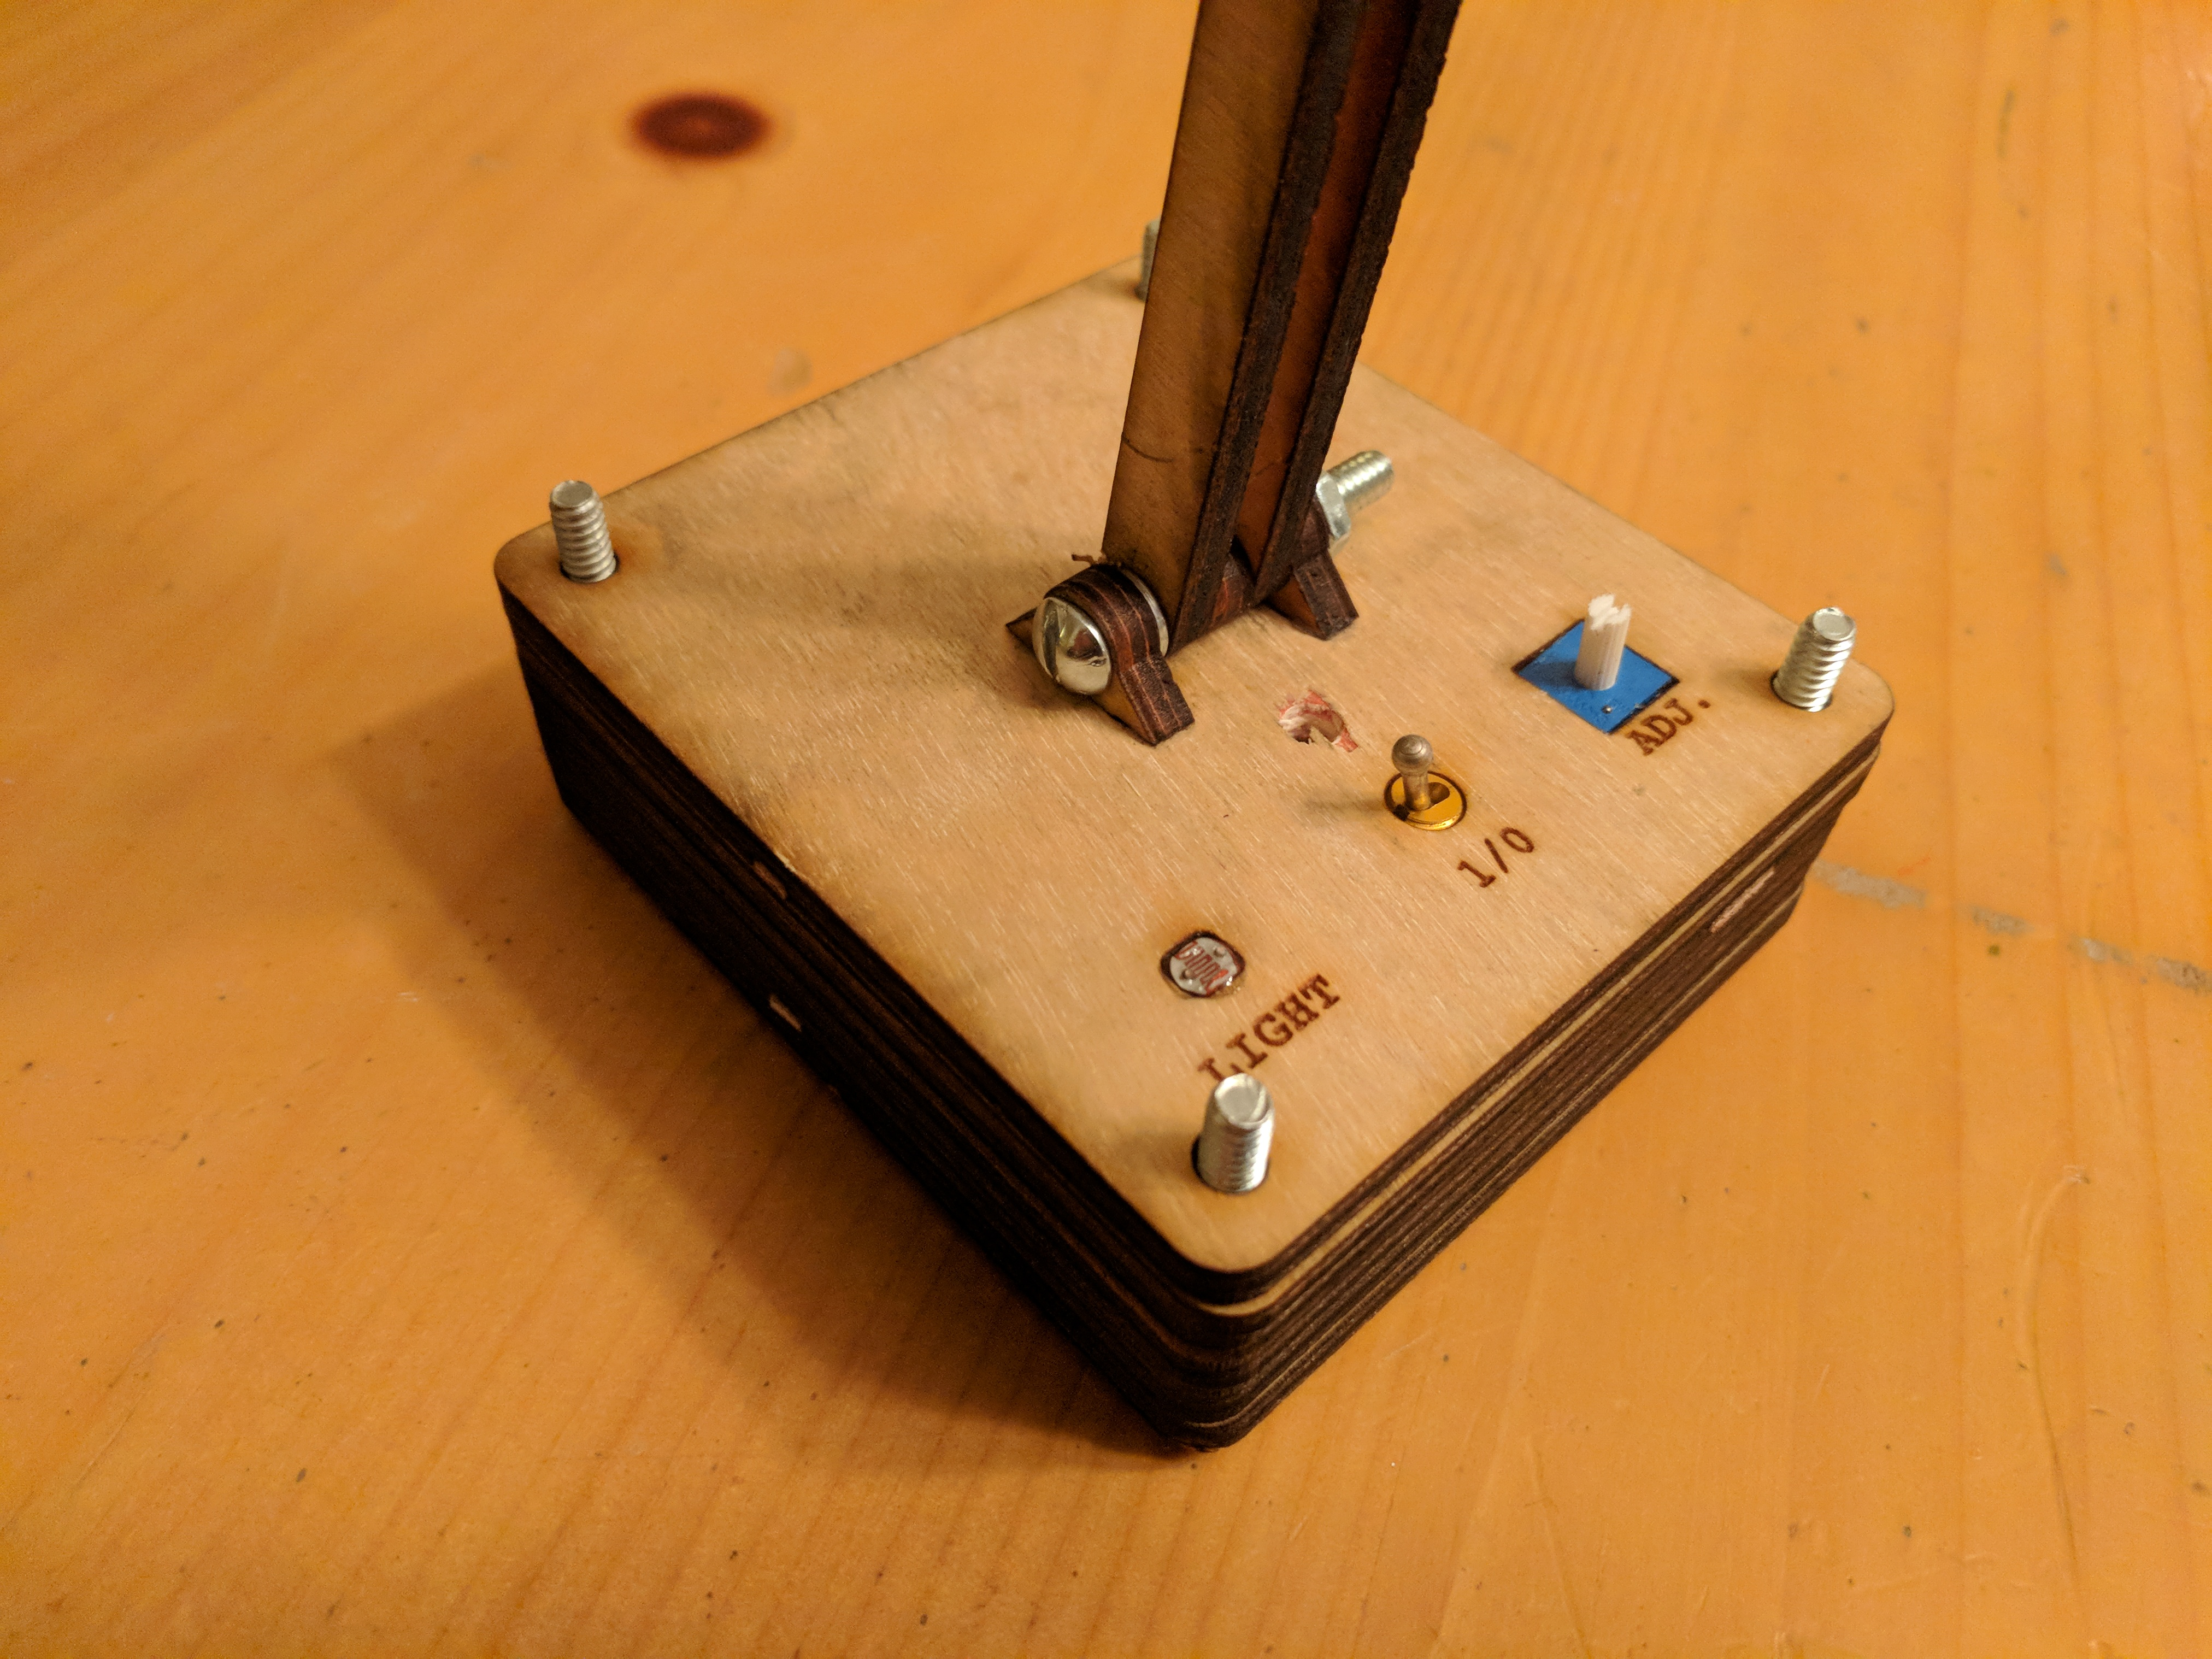
\includegraphics[width=.75\linewidth]{lamp12.jpg}}
\caption{This is the completed base with minimal electronic components in place}
\end{figure}

\end{document}
